\documentclass[12pt]{article}
\usepackage{geometry}
\setlength{\parindent}{0pt}
\geometry{left=1in, right=0.75in, top=1in, bottom=1in}
\newcommand{\Problem}{D}
\newcommand{\Team}{2105432}
\newcommand{\hiddensection}[1]{
\stepcounter{section}
\section*{\Roman {section} \hspace{1em}{#1}}}
\usepackage{newtxtext}
\usepackage{amsmath,amssymb,amsthm}
\usepackage{newtxmath}
\usepackage{graphicx}
\usepackage{xcolor}
\usepackage{fancyhdr}
\usepackage{lastpage209}
\usepackage{multirow}
\usepackage{subfigure}
\usepackage{wrapfig}
\usepackage[utf8]{inputenc}
\usepackage{listings}
\usepackage{xcolor}

\lhead{Team \Team}
\rhead{}
\cfoot{}
\newtheorem{theorem}{Theorem}
\newtheorem{corollary}[theorem]{Corollary}
\newtheorem{lemma}[theorem]{Lemma}
\newtheorem{definition}{Definition}

\begin{document}
	\DeclareGraphicsExtensions{.pdf,.jpg,.tif,.bmp,.png}
	\thispagestyle{empty}
	\vspace*{-16ex}
	\centerline{\begin{tabular}{*3{c}}
	\parbox[t]{0.3\linewidth}{\begin{center}\textbf{Problem Chosen}\\ \Large \textcolor{red}{\Problem}\end{center}}
	& \parbox[t]{0.3\linewidth}{\begin{center}\textbf{2021\\ MCM/ICM\\ Summary Sheet}\end{center}}
	& \parbox[t]{0.3\linewidth}{\begin{center}\textbf{Team Control Number}\\ \Large \textcolor{red}{\Team}\end{center}}	\\
	\hline
\end{tabular}}
{\textbf{}}\\\\
There's always some evolution on music behind the auditory fest, and so are the cooperative effort of musicians across the generations behind the evolution of this great component of the society. Many artists have claimed that they got inspired by the artists of the same or different genre(s), making their works more popular and refreshing the overall atmosphere of music composing globally.\\[2ex]
To explore the influence of the music, our team established a \textbf{Network Model} and analyzed the influence processes of musical evolution that occurred over time in one genre, making full use of the concerto provided by \textbf{PageRank Algorithm}. Moreover, this network model stood out when analyzing how our work express information about cultural influences of music in time or circumstances.\\[2ex]
To find out the influence of music on the albums of the youngsters, our team established a {\textbf{Principal Component Analysis Model}}, having succeeded in finding the principal indicators for measuring the similarity between the artists or songs both within and beyond the genre and discovering whether the objects in the same genre possess more similarities. The model contains {\textbf{Correlation Analysis, Hierarchical Analysis and Factor Analysis}}, analyzing the similarity on the angle of artists and their works respectively.\\[2ex]
To make the result more accurate, our team employed {\textbf{Cosine Similarity}} to calculate the similarity among genres separately. The cosine similarity, meanwhile, is also made full use of to make comparisons between similarities and influences among and within genres. our team also discovered what distinguishes a genre, and some potential relationship among different genres.\\[2ex]
\textbf{Additional networks} was established to give the identification of whether there are characteristics that might signify revolutions (major leaps) in musical evolution from these data and what artists represent revolutionaries (influencers of major change) in our network. By analyzing the key phases of musical reforms which transformed into turning points on the line chart, our team found networks of at the decades matching the turning points.\\[2ex]
\textbf{A bonus network} was employed for identification of whether the similarity data suggest that the identified influencers actually affect the music created by the followers. Our team have found that the network can also indicate the most contagious factors among all music characteristics when taking influencers and followers of one outstanding artist as an example.\\[2ex]
Our team succeeded in revealing the dynamic influencers and how the genres and artists changed over time by establishing another {\textbf{rich-in-chart model}} conducted by the solo of analysis on provided stats.\\[2ex]
The analysis on strengths and weaknesses of the models our team have built and the accuracy of them came up, analyzing the sensitivity of what our team have constructed, proving the stability of all above.\\[2ex]
Finally our team issued a one-page document to the ICM society, our supervisor, about the value of using our approach to understanding the influence of music through networks. The document will also contain how our work would change with more or richer data.\\[2ex]
\textbf{Keywords:} Influencing Network, In(ter)-genre Similarity, Musical Evolutions
\clearpage
\pagestyle{fancy}
\newpage
\setcounter{page}{1}
\rhead{Page {\textbf{\thepage}} of \pageref{LastPage}}
\tableofcontents
{\textbf{}}\\[2ex]
{\textbf{Notice:} All figures in the solution play critical roles in our analysis. Please enlarge them for details if necessary.}
\clearpage
\section{Introduction}
\subsection{Background}
The past centuries worldwide have enjoyed an auditory fest of evolution of music. Many artists compose their tracks according to the heritage of the past generations, some novel instruments, and some external circumstances, exploring their preferred characteristics of their works. All these shifts and revolutions can be regarded as a concert of efforts conducted by both influencers and the followers. By studying the networks of songs and their musical characteristics, our team can get hold of the effects brought by the influencers of the songs' origins.\\[2ex]
Our team was identified by the supervisor to develop a set of models which is able to measure musical influence. Our team should employ the provided data and later claim the value of our approaches.
\subsection{Restatements of the Problem}
The problem should be translated into the following tasks which requires to be finished:
\begin{itemize}
	\item Create network(s) for the musical influences. Figure out the parameters of the influence and what they reveal.
	\item Use the statistics provided to explore the indicators to measure the similarity of music, analyzing the similarities between artists of the same and various genres simultaneously.
	\item Compare similarities and influences between and within genres and exploring the distinctions among genres.
	\item Indicate whether the similarity data, as reported in the data set \textit{data\_influence}, suggest that the identified influencers in fact influence the respective artists. 
	\item Identify whether there are characteristics that might signify revolutions (major leaps) in musical evolution from these data and what artists represent revolutionaries (influencers of major change) in your network.
	\item Analyze the influence processes of musical evolution that occurred over time in one genre and find the indicators which can reveal the influencers dynamically.
	\item Exploring for how our work express the information about influence of music in time or circumstances.
\end{itemize}
\clearpage
\subsection{Our Work}
\begin{figure}[h]
\centering
	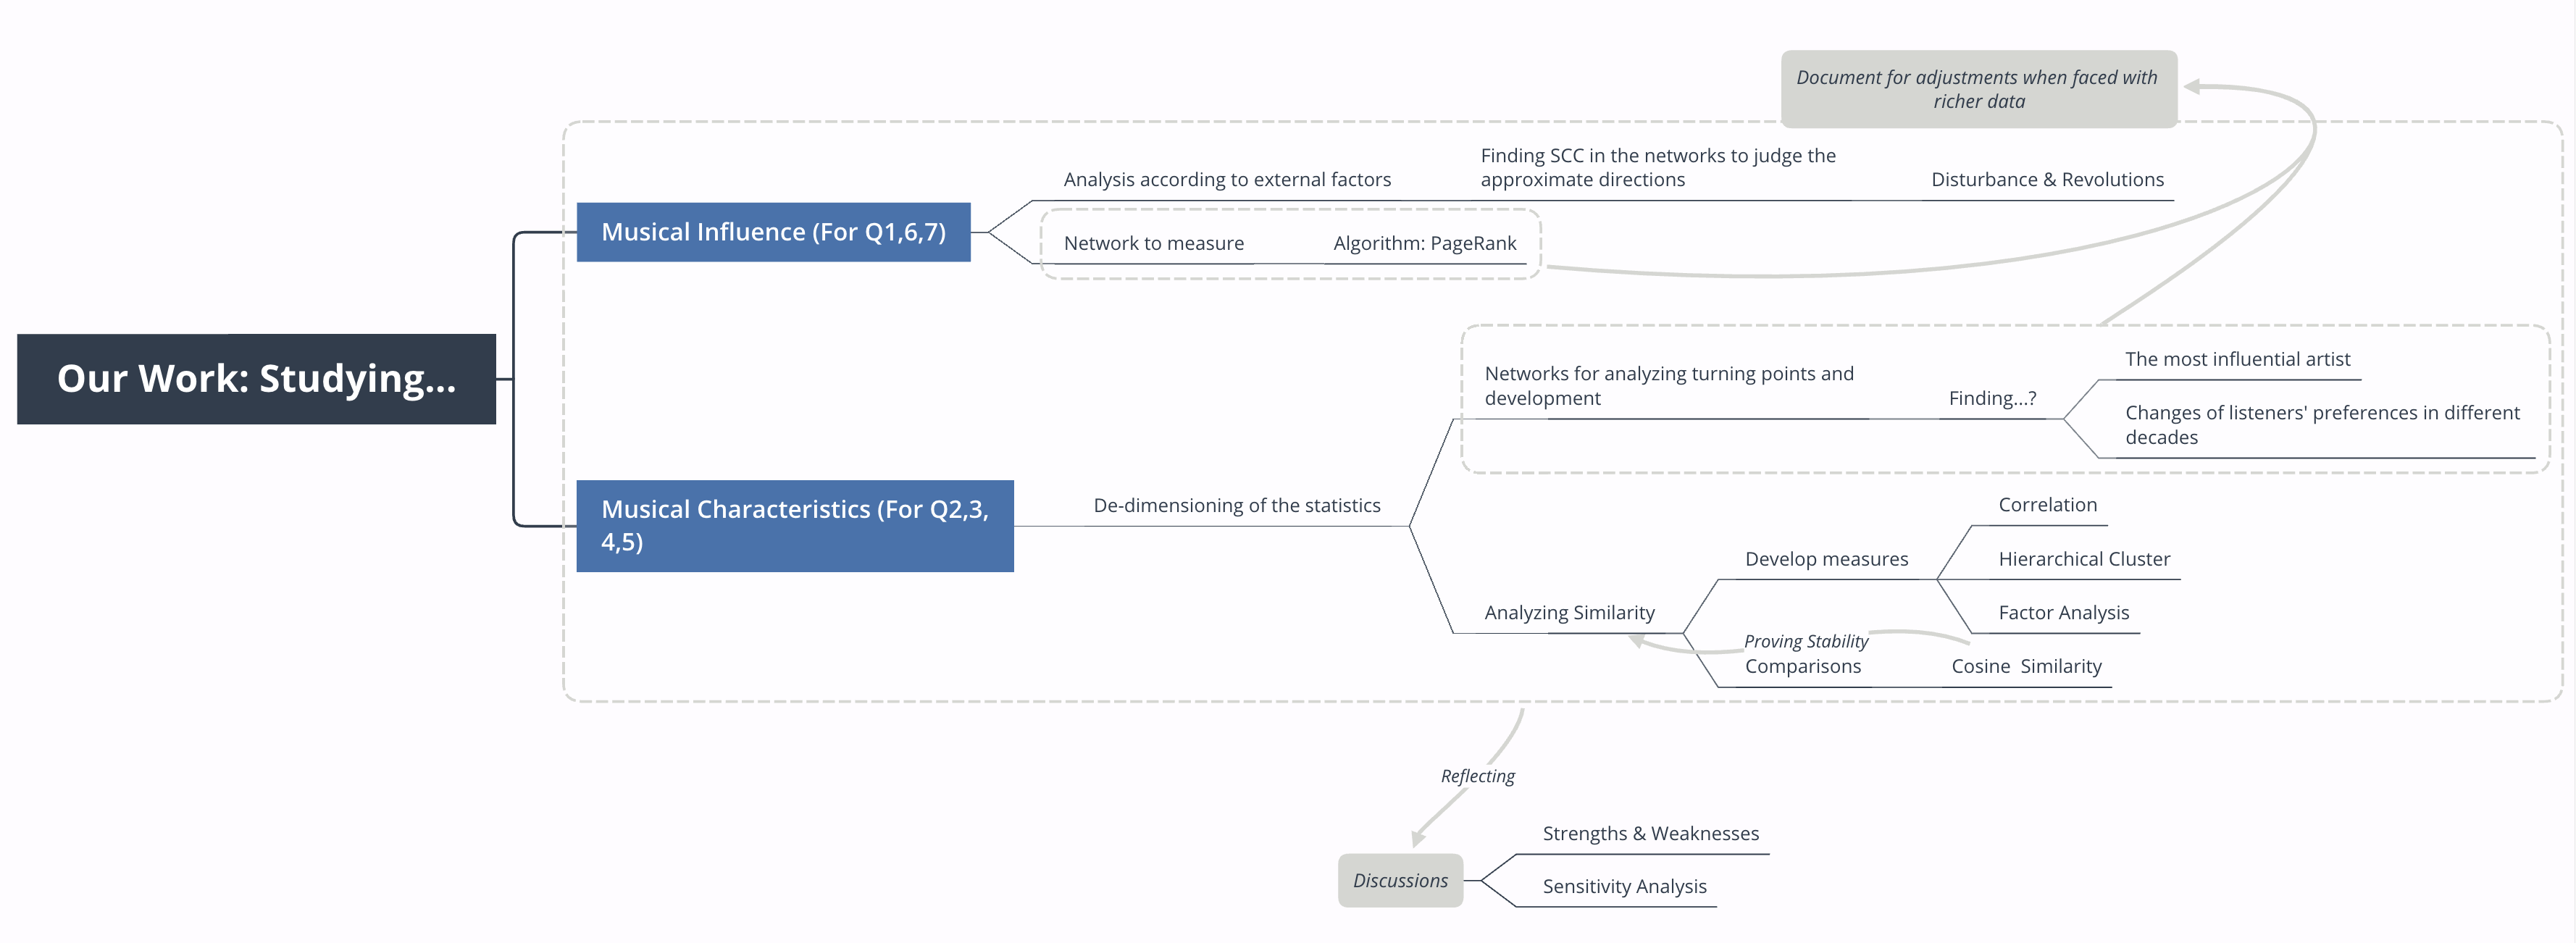
\includegraphics[scale=0.27]{Music24.png}
	\caption{Sketch Map of The Works of Our Team}
\end{figure}
\section{Assumptions}
\begin{itemize}
	\item The preferences of people with regard to music will not change greatly in a short time. In other words, popularity during other phases still stands the test of references.
	\item The overall trend of the musical market will remain stable.
	\item The sudden factors will leave no strike on the operation of models.
	\item Influencers of one artist feature different impacts on others. The more influential the influencer is, the more impact it conveys to his followers.
	\item Artist may take an active role in making a shift towards their own musical characteristics.
\end{itemize}
\clearpage
\section{Model 1: Network Model for Musical Influence}
\begin{table}[htp]
\centering
	\begin{tabular}{|c|c||c|c|}
	\hline
		Parameters &Definitions &Parameters &Definitions\\
		\hline
		$V$ & Sets of Dots &$deg_{out}(u)$ &Out-degree of the Node $u$\\
		$E$ & Sets of Directed-Edges & $deg_{in}(u)$ &In-degree of the Node $u$\\
		$G(V,E)$ & Network Composed by $V$ and $U$ &$PR(u)$ & PageRank Value of the Node $u$\\
		$(u,v)$ & Directed-Edge Connecting $u$ and $v$ &$q$ & Damping Factor\\
		$|V|$ &Size of $V$ &$|E|$ &Size of $E$\\
		$t$&Times of Running PageRank Algorithm &$G^{'}(V^{'},E^{'})$ &Network By Shrinking $G(V,E)$\\
		$V'$&Sets of Dots Got By Shrinking $V$ &$|V'|$&Size of $V$\\
		$E'$&Sets of Edges Got By Shrinking $E$ &$|E'|$&Size of $E$\\
		\hline
	\end{tabular}
\end{table}
The model is aimed at solving {\textbf{Problem 1, 6 and 7}} in the restatements, basing on the {\textbf{Assumption 4 and 5}}. 
\subsection{Network for Indicators of Musical Influences}
The algorithm of PageRank, initially, will grant the nodes with the same value of PageRank. During each phase of the calculation, the equation
\begin{equation*}
PR(u)=\sum_{(v,u)\in E}\frac{PR(v)}{deg_{out}(v)}
\end{equation*}
will be the rule when the node $u$ distributes $PR(u)$ evenly to all his followers and makes a sum on the PageRank Value inherited from his influencers, which in turn triggers a new round of PageRank. The terminal PageRank occur when there's no change on PageRank of every node within the permission of the inaccuracy.\\[2ex]
Existence of nodes of which the $deg_{out}$ is 0 is inevitable. They may be affected by other factors which have nothing to do with the artists, so our team have to introduce the dumping factor to minimize the effect.\\[2ex]
$$PR(u)=(1-q)+q\cdot\sum_{(v,u)\in E} \frac{PR(v)}{deg_{out}(v)}$$
Generally, state-transition matrix is required for the calculation of the new value of $PR$.\textcolor{blue}{$^{[1]}$}\\[2ex]
This network is purposed for \textbf{Problem 1} in the restatements. Our team established a directed network $G(V,E)$, where every node represents one artist and each of the directed-edge $(u,v)$ symbolizes one relationship of influence ($u$ for influencer, while $v$ for follower). The network will display the influential network among the post-1960s artists.\\[2ex]
The indicators of musical influences are as follows:\textcolor{blue}{$^{[2]}$}
\begin{itemize}
	\item Degree Centrality ({\textsc{dc}}): The more the size of one node's out-degree in the network is, the more influential the artist at this node is.
	\item Betweenness Centrality ({\textsc{bc}}): The more the frequency of the node which exists on the shortest route between 2 other nodes is, the more influential the artist at this node is.
\end{itemize}

\begin{wrapfigure}{l}{0cm}
	\centering
	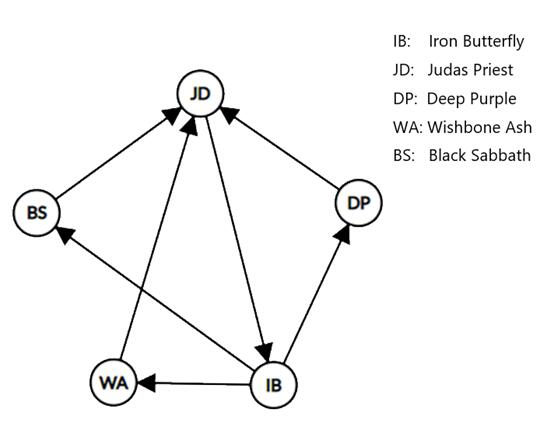
\includegraphics[scale=0.5]{Music7}
	\caption{Sub-Network of the Active Artists in the 1960s}\
\end{wrapfigure}
Our team consider the following sub-network where all nodes represent artists who became active in the 1960s, making the use of the PageRank Algorithm to find the artists who, in the whole network, are playing the most crucial role.\\[2ex]
In the sub-network, {\textit{Iron Butterfly}} represents the node which are quite critical according to {\textsc{dc}}, while those got from {\textsc{bc}} are named {\textit{Iron Butterfly}} and {\textit{Judas Priest}} respectively.\\[2ex]
Our team then run the Algorithm of PageRank and discovered that the nodes follow the relationship {\textit{Iron Butterfly} > \textit{Black Subbath} = \textit{Deep Purple} = \textit{Wishbone Ash} > \textit{Judas Priest}} in the order of PageRank. The larger the value of PageRank the artist possesses, the more influential he is on the nodes.\\[2ex]
As a result, it's obvious to say that {\bfseries{the most influential node is {\textit{Iron Butterfly}}}}.\\
\subsection{Analysis on Impacts Conducted By Revolutions}
The model is aimed at solving {\textbf{Problem 6}} in the restatements.\\[2ex]
Our team measure the musical characteristics by making out the average of the music characteristics of one artist. Take the genre $Country$ as an example. Our team depicted the characteristics in the same chart and succeeded in supervising the trend of musical characteristics from the 1960s to the 2010s.\\[2ex]
The stacked column of musical characteristics are as follows.

\begin{wrapfigure}{l}{0cm}
\centering
	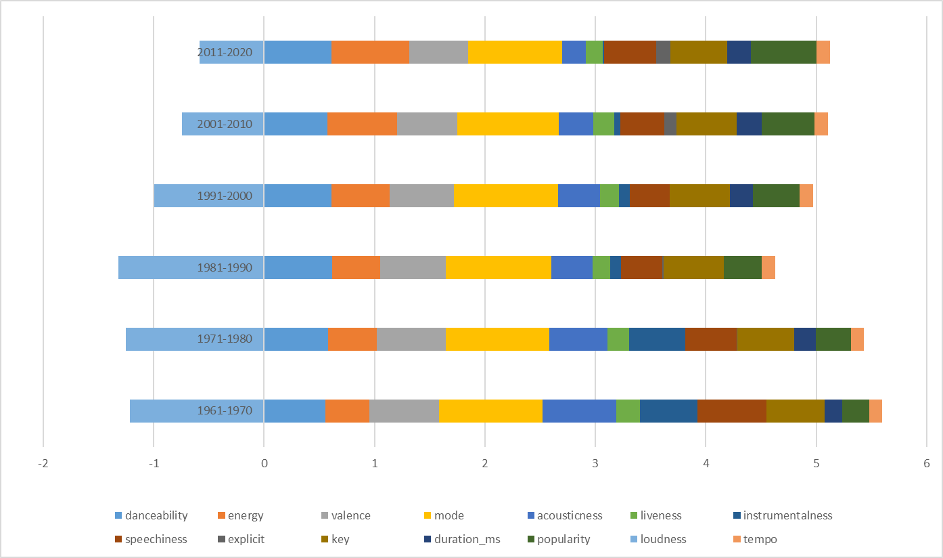
\includegraphics[scale=0.556]{Music9}
\end{wrapfigure}

It implies that {\textbf{instrumentalness has dropped and so has acousticness since the 1980s.} In other words, instruments and acoustics have been increasingly absorbed into the genre {\textit{Country}}. This may be attributed to the widespread development of computer. Similarly, indicators related to technology, such as {\textit{instrumentalness}} and {\textit{acousticness}}, may mirror the influence the technology has on music. The stable increase happening on \textit{energy} can be originated from the 1960s thanks to the rising level of living citizens after WWII. The diversification of description also give rise to the increase of it.
\subsection{Identification on Impacts Brought By External Factors}
\subsubsection{Model for Spread of the Influence on the Network Basing on \textsc{scc}}
\textsc{scc} is the abbreviation of Strongly Connected Components.\\[2ex]
Our team established \textsc{scc} in the directed map so that every node in the components can be influenced by each other. As is shown in figure (a) below, node 1, 2, 3, 4 and 5 are components of one \textsc{scc} which is marked as \textsc{a}, while node 6, 7 and 8 makes up \textsc{scc b}. \\[2ex]
Our team found all \textsc{scc} by Tarjan Algorithm and depicted a directed acyclic graph on the basis of the initial chart by regarding every \textsc{scc} as a node.\textcolor{blue}{$^{[3]}$}
\begin{figure}[h]
\centering
	\begin{subfigure}[Sketch Map of \textsc{scc}]
		{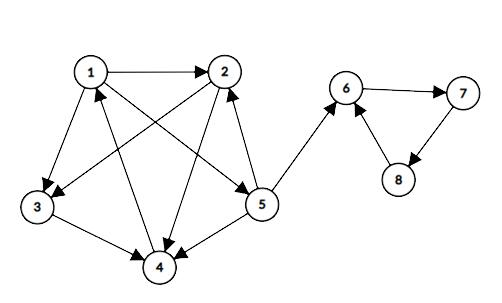
\includegraphics[scale=0.3]{Music19}}
	\end{subfigure}
	\hspace{2cm}
	\begin{subfigure}[Sketch Map of Shrink Point]
		{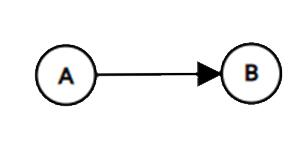
\includegraphics[scale=0.6]{Music20}}
	\end{subfigure}
\caption{Sketch Maps With \textsc{scc}}
\end{figure}\\
In the acyclic graph, music characteristics of every node are the average value of those of the nodes in the \textsc{scc}.
\subsubsection{Model for Examining External Disturbance on the Network}
Our team can discover the approximate directions of spread and the origin of the influence by sorting the acyclic graphs topologically \footnotemark\ .
\\[2ex]
Our team added directed-edges to the network dynamically in the order of time according to the time when the follower turn active in every relationship of influences. Simultaneously, our team maintain the \textsc{scc} in the network and shrink them to \textsc{dag} according to Incremental Strongly Connected Components Algorithm.\textcolor{blue}{$^{[4]}$} The moment when changes in the stats at the node whose in-degree is 0 in \textsc{dag} turn obvious should indicate the possibility that external factors have left influences on the network.
\footnotetext {Topological sorting\textcolor{blue}{$^{[5]}$} runs on the following basis:
\begin{itemize}
	\item Every node is included in the pattern and should appear for only once.
	\item Route from B to A should not exist if the node A stands in the front of the node B.
\end{itemize}
}
\clearpage
\section{Model 2: Model for Analyzing Musical Characteristics}
\begin{table}[htp]
\centering
	\begin{tabular}{|c|c||c|c|}
		\hline
		Parameters & Definitions & Parameters & Definitions\\
		\hline
		$D_{i,1}$ & Danceability& $I_i$ &Instrumentalness\\
		$E_{i,1}$ &Energy&$L_{i,2}$ &Liveness\\
		$V_i$ &Valence&$S_i$ &Speechness\\
		$T_i$ &Tempo&$E_{i,2}$ &Explicit\\
		$L_{i,1}$ &Loudness&$D_{i,2}$ &Duration ms\\
		$M_i$ &Mode&$P_i$ &Popularity\\
		$s_n$ &Comprehensive Score of Artist&$Y_i$ &Year\\
		$A_i$ &Acoustics &$K_i$ &Key\\
		$R$ &Constant for Correlation&&\\
		\hline
	\end{tabular}
\caption{Parameters and Their Definitions}
\end{table}
The model is purposed at solving {\textbf{Problem 2, 3, 4 and 5}} issued in the restatement, basing on the {\textbf{Assumption 1,2 and 3}}.our team take the characteristics of music as significant indicators to measure the similarity among different works of music. We analyzed influences of artists from a different angle.\\[2ex]
Our team discover the major influencers by employing the {\textbf{Analytic Hierarchy Process, Factor Analysis and Entropy weight Method, etc.}}\\
\subsection{Sub-Model for Developing Measures of Music Similarity}
Our team use this sub-model to solve \textbf{Problem 2} in the restatements. By using the measure, our team can find it easy to find out whether the artists within genre are more similar than artists between genres.
\subsubsection{Correlation Analysis}
Our team initially introduced the Spearman Constant
\begin{equation}
	r_s=1-\frac{6\sum\limits_{i=1}^nd_i^2}{n(n^2-1)}.
\end{equation}
In the equation above, $d_i$ represents the rank differences of the two data $X_i$ and $Y_i$, which originates from the data sets $X$ and $Y$. The rank of one datum should be the position of it after putting them in min-to-max order. It can also be proved that $r_s$ can vary in the set [-1,1].\\[2ex]
Figure 3(a) displays the value of the Spearman Constant with the help of the lightness of the color in each block.
The heat map also illustrated the fact that {\textbf{Energy, Loudness, Acoustics and Year are the strongest factors backing the stage of popularity.}}\\[1ex]
Our team then introduced Kendall's tau-b Constant of Correlation, {\textsc{ktcc}}, to prove the accuracy of the previous discoveries under the music of Spearman Constant, making the heat map in a similar way and can be seen on Figure 3(b).\\
\begin{figure}[htbp]
	\centering
	\subfigure[Heat Map of $r_s$]{
	\label{figa}
	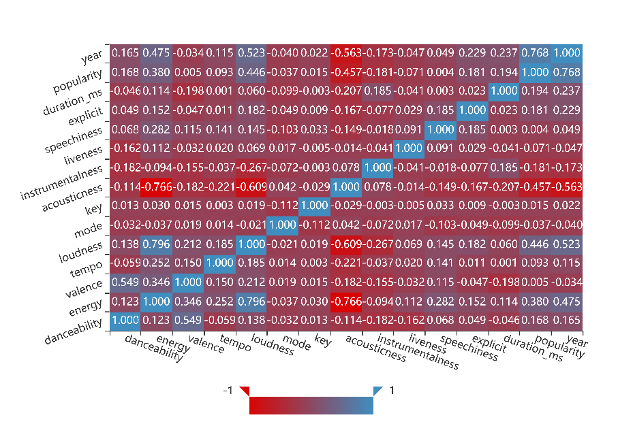
\includegraphics[height=3cm]{Music1}}
	\hspace{0.5cm}
	\subfigure[Heat Map of {\textsc{ktcc}}]{
	\label{fig:subfig:b}
	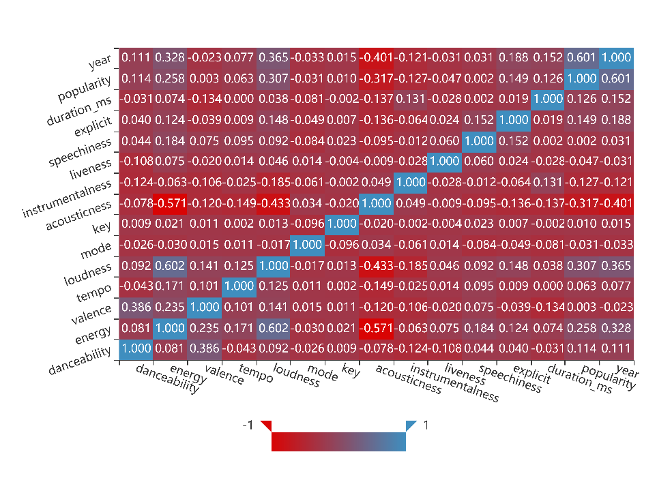
\includegraphics[height=3cm]{Music2}}
	\subfigure[Heat Map of {\textsc{fl}}]{
	\label{fig:subfig:c}
	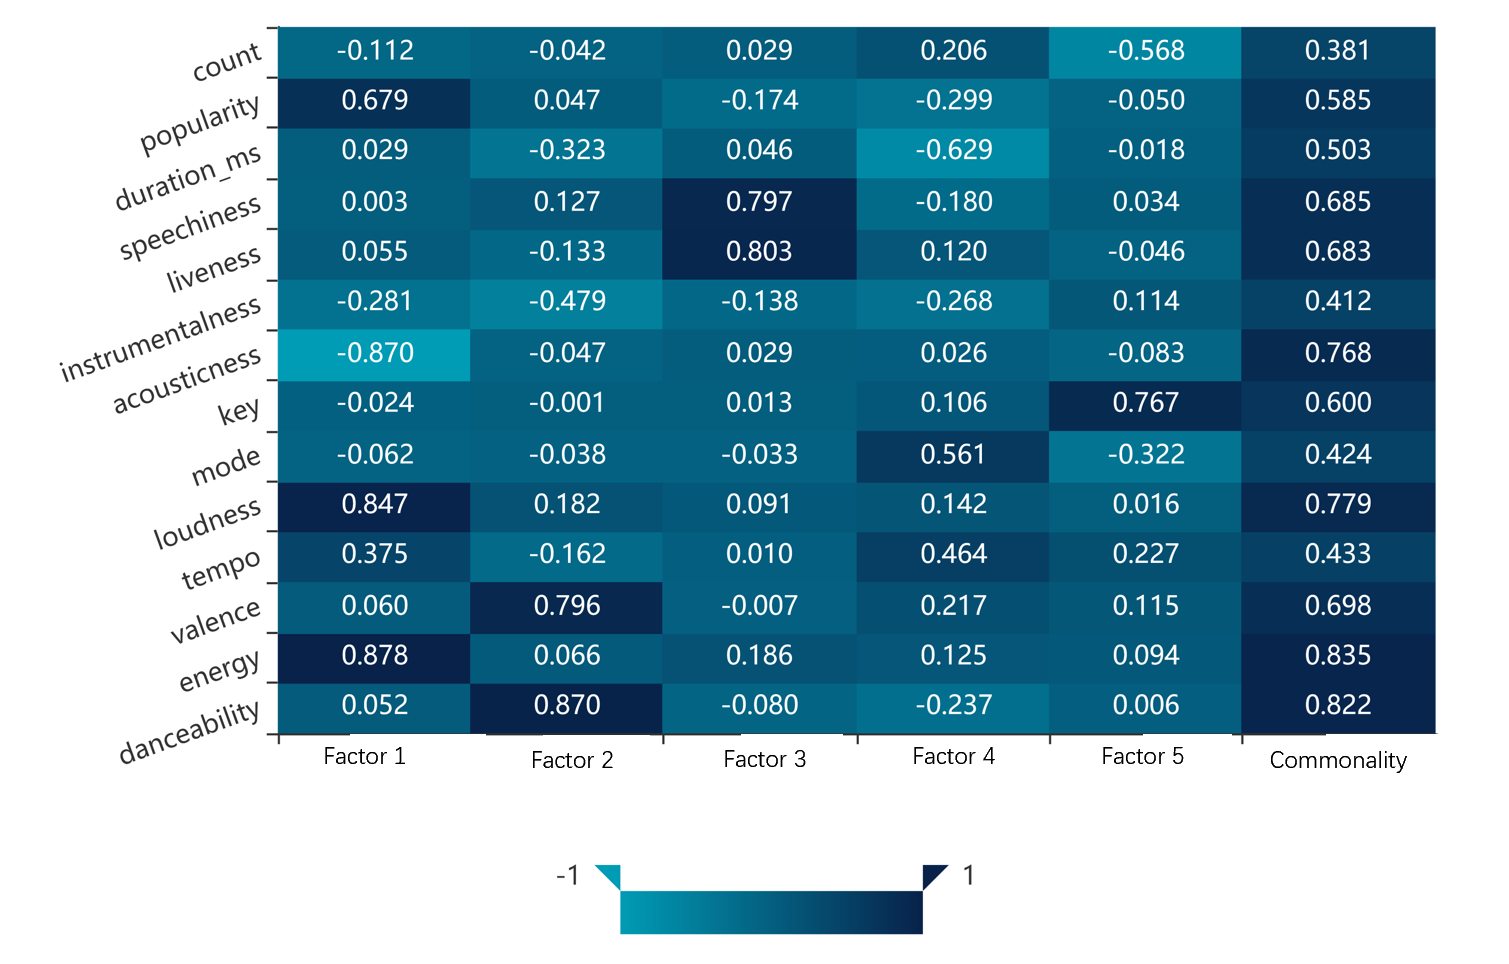
\includegraphics[height=2.8cm]{Music3}}
	\caption{Heat Maps of Different Measures}
\end{figure}
\\We've discovered that the heat maps, (a) and (b), have succeeded in striking a chord with each other.
\subsubsection{Hierarchical Cluster Analysis}
\begin{wrapfigure}{l}{10cm}
\centering
	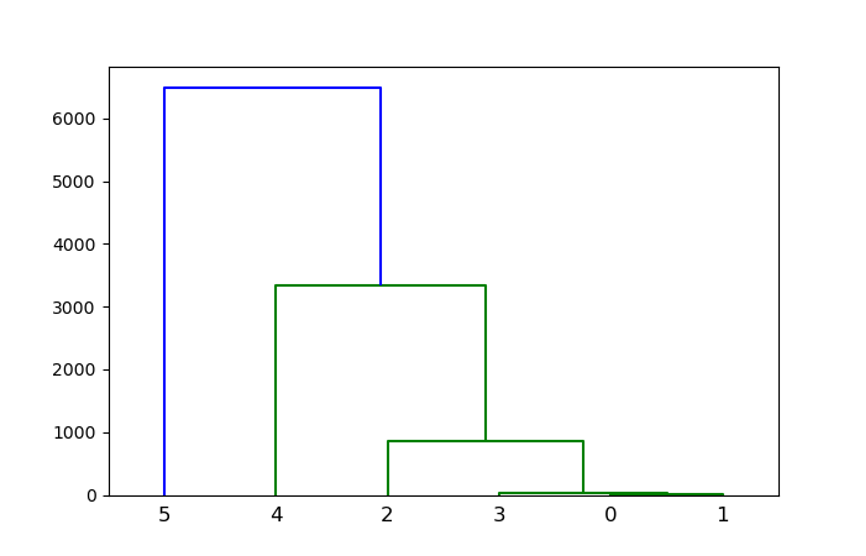
\includegraphics[scale=0.5]{Music6}
	\end{wrapfigure}
To simplify the influencing factors of the problem, we will only discuss the principal components figured out in the subsection {\textbf{4.1}}.\\[2ex]
Hierarchical cluster analysis features 3 types, Single Linkage, Complete Linkage and Average Linkage included. Our team chose the last one due to the fact that it can fit our model more perfectly.\textcolor{blue}{$^{[6]}$}\\[2ex]
Our team then got the following chart and table with the help of our calculation.\\
\begin{table}[h]
	\centering
	\begin{tabular}{|c|c|c|c|c|c|c|}
	\hline
	 \multirow{2}{*}{Types} &\multicolumn{3}{c|}{1} &2 &3 &4\\
	 \cline{2-7}
	 &Danceability &Energy &Acoustics &Loudness &Popularity &Count\\
	 \hline
	 Peak & 0.072 &-0.599 &-0.909 &2.934 &0.523 & 78.903\\
	 Skewness & -0.230 &-0.267 &0.592 &-1.106 &-0.507 & 7.333\\
	 {\textsc{cv}} &0.248 &0.369 &0.858 &-0.420 &0.334 &2.293\\
	 \hline
	\end{tabular}\\
{\textsc{cv}}:Coefficient of Variation
\caption{Explanation of Some Components in the Tree Chart Above}
\end{table}

\subsubsection{Factor Analysis}
Our team calculated, making full use of the duet conducted by KMO Test and Bartlett Test, to discover that the parameters shown in the problems meet the demands of the conduction of Principal Component Analysis. Our team then can get Total Variance explained as follows.\\
\begin{table}[htbp]
{\centering
	\begin{tabular}{|c|c|c|c|c|c|c|}
		\hline
		\multirow{2}{*}{Factor Number} & \multicolumn{3}{c|}{Eigenvalue} &\multicolumn{3}{c|}{Percentage of Variance After Rotation}\\
		\cline{2-7}
		&Eigenvalue &{\textsc{pv}} &Total & Eigenvalue &{\textsc{pv}} & Total\\
		\hline
		1 &3.713 &24.757\% &24.757\% &2.987 &19.916\% &19.916\%\\
		\hline
		2 &1.646 &10.971\% &35.727\% &1.844 &12.293\% &32.209\%\\
		\hline
		3 &1.336 &8.904\% &44.631\% &1.715 &11.436\% &43.645\%\\
		\hline
		4 &1.200 &8.000\% &52.631\% &1.309 &8.727\% &52.372\%\\
		\hline
		5 &1.119 &7.459\% &60.090\% &1.158 &7.718\% &60.090\%\\
		\hline
		6 &0.992 &6.616\% &66.706\%\\
		\cline{1-4}
		7 &0.938 &6.250\% &72.956\%\\
		\cline{1-4}
		8 &0.830 &5.532\% &78.489\%\\
		\cline{1-4}
		9 &0.798 &5.319\% &83.807\%\\
		\cline{1-4}
 		10 &0.741 &4.937\% &88.744\%\\
		\cline{1-4}
		11 &0.663 &4.417\% &93.161\%\\
		\cline{1-4}
		12 &0.373 &2.487\% &95.648\%\\
		\cline{1-4}
		13 &0.329 &6.616\% &97.843\%\\
		\cline{1-4}
		14 &0.204 &1.357\% &99.201\%\\
		\cline{1-4}
		15 &0.120 &0.799\% &100.000\% \\
		\cline{1-4}
		\end{tabular}\\
}
{\textsc{pv}}: Percentage of Variance
\caption{Total Variance Explanation Table}
\end{table}
It's universally acknowledged that the higher the {\textsc{pv}} is, the more important role the factor is playing. The statistics after rotation can also work when solving the formula of principal components.\\[2ex]
Our team take the the top 5 in the list as principal components because the eigenvalue has dropped below 1 after the Factor Number turns more than 6.\\[4ex]
Our team then draw the Nightingale Rose-Chart and the Scree Chart to describe the extent to which the influences the principal components have on statistics. The amount of principal components which require to be chosen can be reflected by the slope of the drop on eigenvalue and can be adjusted according to Table 3.\\[2ex]
\begin{figure}[htbp]
\centering
\subfigure[Nightingale Rose Chart]{
	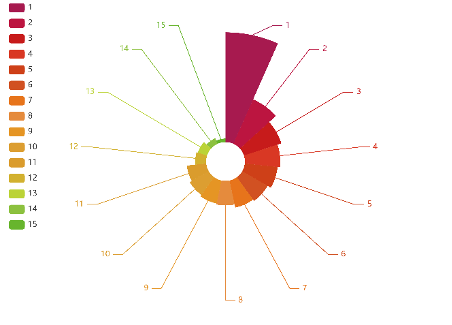
\includegraphics[scale=0.7]{Music4}}
\subfigure[Scree Chart]{
	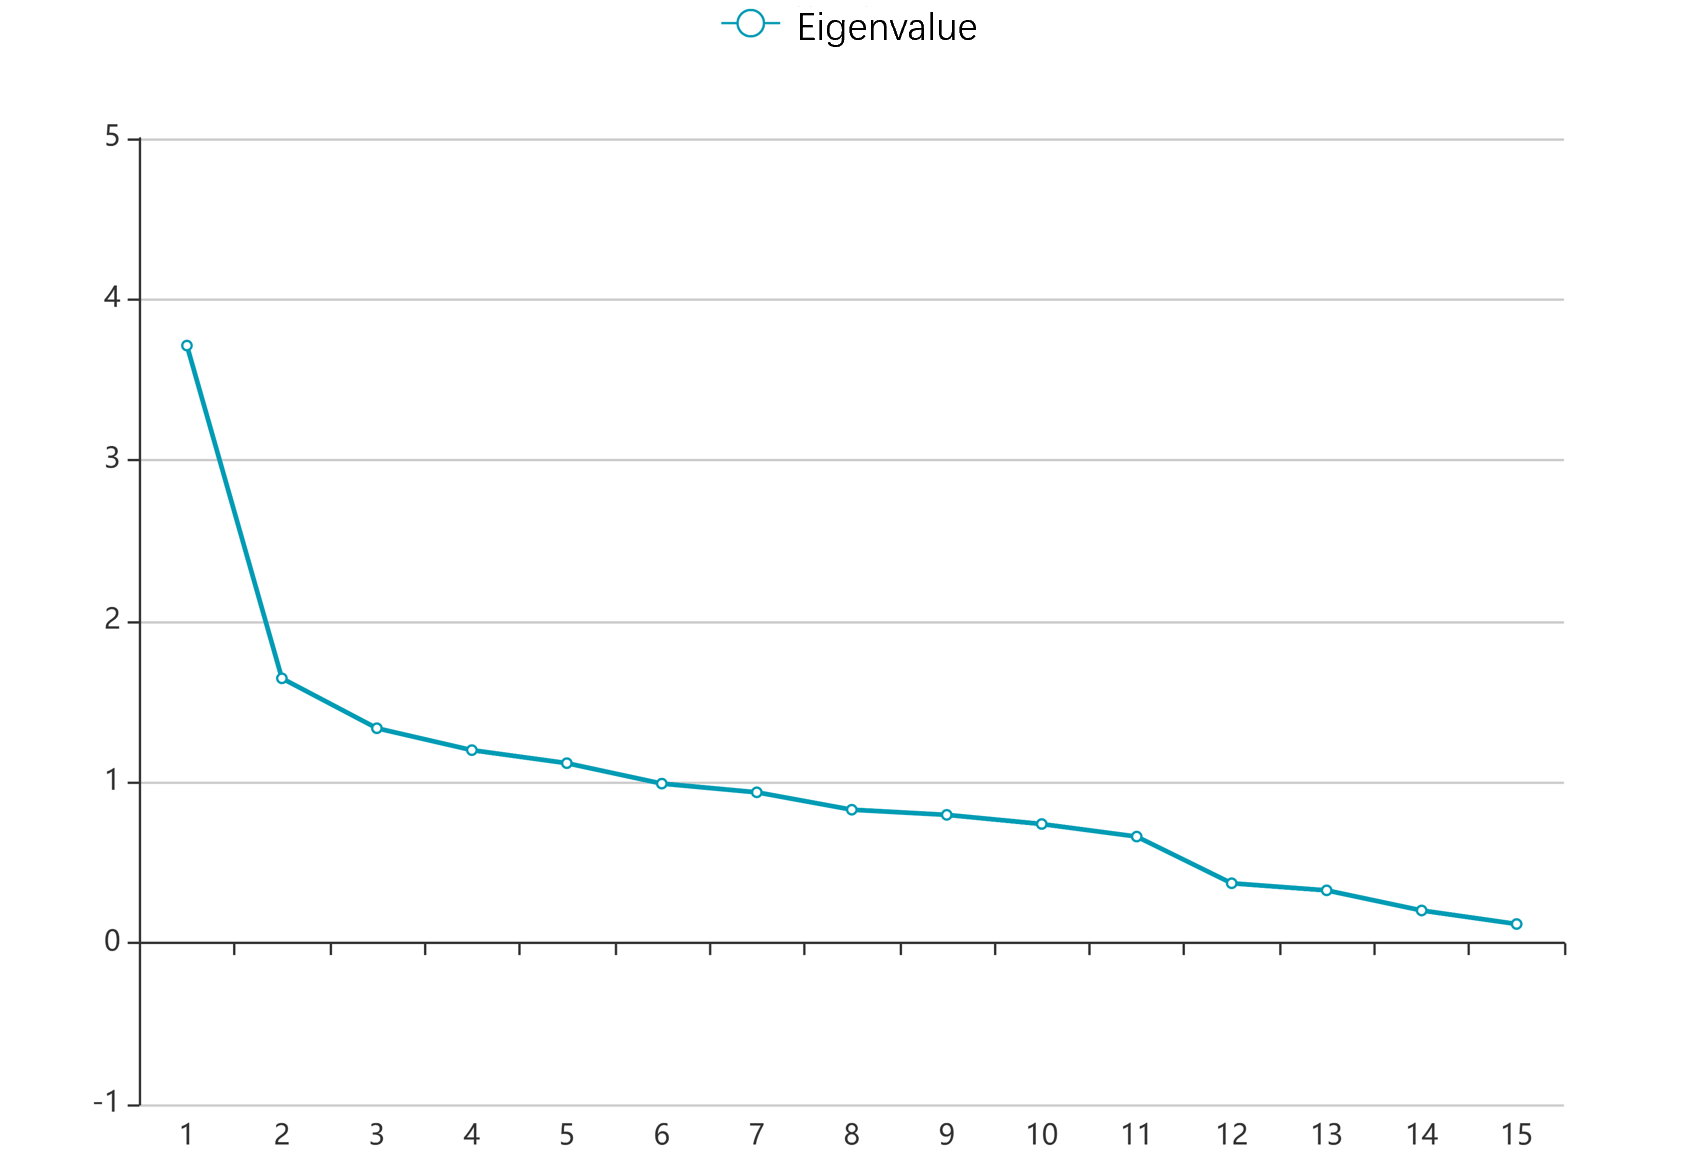
\includegraphics[scale=0.1]{Music5}}
	\caption{Charts to Find the Principal Components}
\end{figure}\\
Next, our team analyzed the significance of the potential variables with the heat map of factor loading shown in Figure 3(c). The nearer the value is to the 1 or $-1$, the more important the potential factors are.\\[2ex]
Our team then are able to induce the formula of the model as follows.
\begin{equation}
F_i=\alpha_i D_{i,1}+\beta_i E_i+\gamma_i V_i+\delta_i T_i+\epsilon_i L_{i,1}+\zeta_i M_i+\nu_i K_i+\xi_i A_i+\kappa_i I_i+\pi_i L_{i,2}+\rho_i S_i+\sigma_i E_{i,2}+\eta_i D_{i,2}+\theta_i P_i+\iota_i Y_i
\end{equation}
The value of $i$ and its matching parameters in the equation (2) are shown below. All parameters but for $i$ have multiplied by 1000.\textcolor{blue}{$^{[7]}$}
\begin{table}[htp]
\centering
\begin{tabular}{|c||c|c|c|c|c|c|c|c|c|c|c|c|c|c|c|}
\hline
$i$ &$\alpha_i$ &$\beta_i$ &$\gamma_i$ &$\delta_i$ &$\epsilon_i$ &$\zeta_i$ &$\nu_i$ &$\xi_i$ &$\kappa_i$ &$\pi_i$ &$\rho_i$ &$\sigma_i$ &$\eta_i$ &$\theta_i$ &$\iota_i$\\
\hline
\hline
	1 &38 &77 &-145 &-89 &128 &-1 &-44 &-169 &-74 &-155 &-58 &182 &58 &358 &359\\
	\hline
	2 &469 &20 &449 &-78 &58 &9 &36 &26 &-200 &-124 &71 &-8 &-279 &-58 &-91\\
	\hline
	3 &-216 &339 &170 &420 &224 &58 &17 &-214 &29 &303 &-50 &-290 &95 &-177 &-138\\
	\hline
	4 &-11 &34 &-70 &-74 &2 &-30 &-2 &67 &-89 &413 &621 &438 &-77 &-69 &-17\\
	\hline
	5 &134 &63 &100 &-51 &-34 &-649 &517 &-69 &232 &-38 &45 &-26 &283 &-42 &-31\\
	\hline
\end{tabular}
\end{table}
\\
Meanwhile, our team can safely reach an equation
\begin{equation}
	F=\frac{199F_1+123F_2+114F_3+87F_4+77F_5}{601}
\end{equation}
to get the comprehensive score of one artist, $F$ in the equation (3), as is displayed in Table 3.\\[2ex]
{\textbf{The lower the value $\delta=|s_1-s_2|$ is, the stronger the link between these 2 scores' owners should be.}
\begin{table}[h]
\centering
\begin{tabular}{|c|c|}
	\hline
	Artist ID &Score\\
	\hline
	674417 & 1.68778\\
	131866 & 1.53988\\
	644216 & 1.43469\\
	... &...\\
	943649 &-1.21662\\
	1768491 &-1.25053\\
	100426 &-1.26898\\
	\hline
	\end{tabular}
	\caption{Rank of Top 3 and Bottom 3 Artists' Comprehensive Score}	
\end{table}
\subsubsection{Result of This Sub-model}
Having combined all discoveries of explorations above, we succeeded in reaching the conclusion that {\textbf{Correlativity among artists of the same genre stands far more obvious than that among artists of various genres. In other words, artists of the same genre feature more similarities than those of inter-genre.}}
\subsection{Sub-model for Comparing Similarities/Influences Between/Within Genres}
This model is aimed at solving \textbf{Problem 3} in the restatements.\\[2ex]
\subsubsection{Cosine Similarity}
Our team mentioned the index $F$ to find out $\delta$, the similarity between the works of music, previously. The $\delta$ between different genres, however, will bring quite significant inaccuracy despite the fact that the absolute difference between their individual values. Thus, for better comparison between similarities and influences between and within genres, we're now introducing the {\textbf{Cosine Similarity}}, {\textsc{cs}}, to solve the problem of the unification among the measurements of the parameters.\\[2ex]
{\textsc{cs}} employs the cosine of the angle of 2 vectors in one certain space to measure the differences between the 2 individuals they represent. {\textsc{cs}} focus on the differences on directions rather than lengths or anything else. It can be calculated in the following way:
\begin{equation}
	sim(X,Y)=\cos\theta=\frac{\boldsymbol{x}\cdot\boldsymbol{y}}{|\boldsymbol{x}||\boldsymbol{y}|}
\end{equation}
Our team have to discuss the $\cos\theta$ on the multi-dimension level thanks to the concert conducted by various factors. It can be calculated in the following equation if the n-dimensional vectors $\boldsymbol{x}$ and $\boldsymbol{y}$ possess the coordination $(x_1, x_2,\cdot\cdot\cdot ,x_n )$ and $(y_1, y_2,\cdot\cdot\cdot ,y_n )$ respectively.
\begin{equation}
	\cos\theta=\frac{\sum\limits_{i=1}^nx_iy_i}{\sqrt{\sum\limits_{i=1}^nx_i^2}\sqrt{\sum\limits_{i=1}^ny_i^2}}
\end{equation}
Having calculated the index $sim$ among genres, our team have discovered that the most significant indicators, which shoulder the most weight, are $D_{i,1}$, $Y_i$ and $A_i$.\textcolor{blue}{$^{[8]}$}
\subsubsection{Similarities Between and Within Genres}
\begin{wrapfigure}{l}{10cm}
\centering
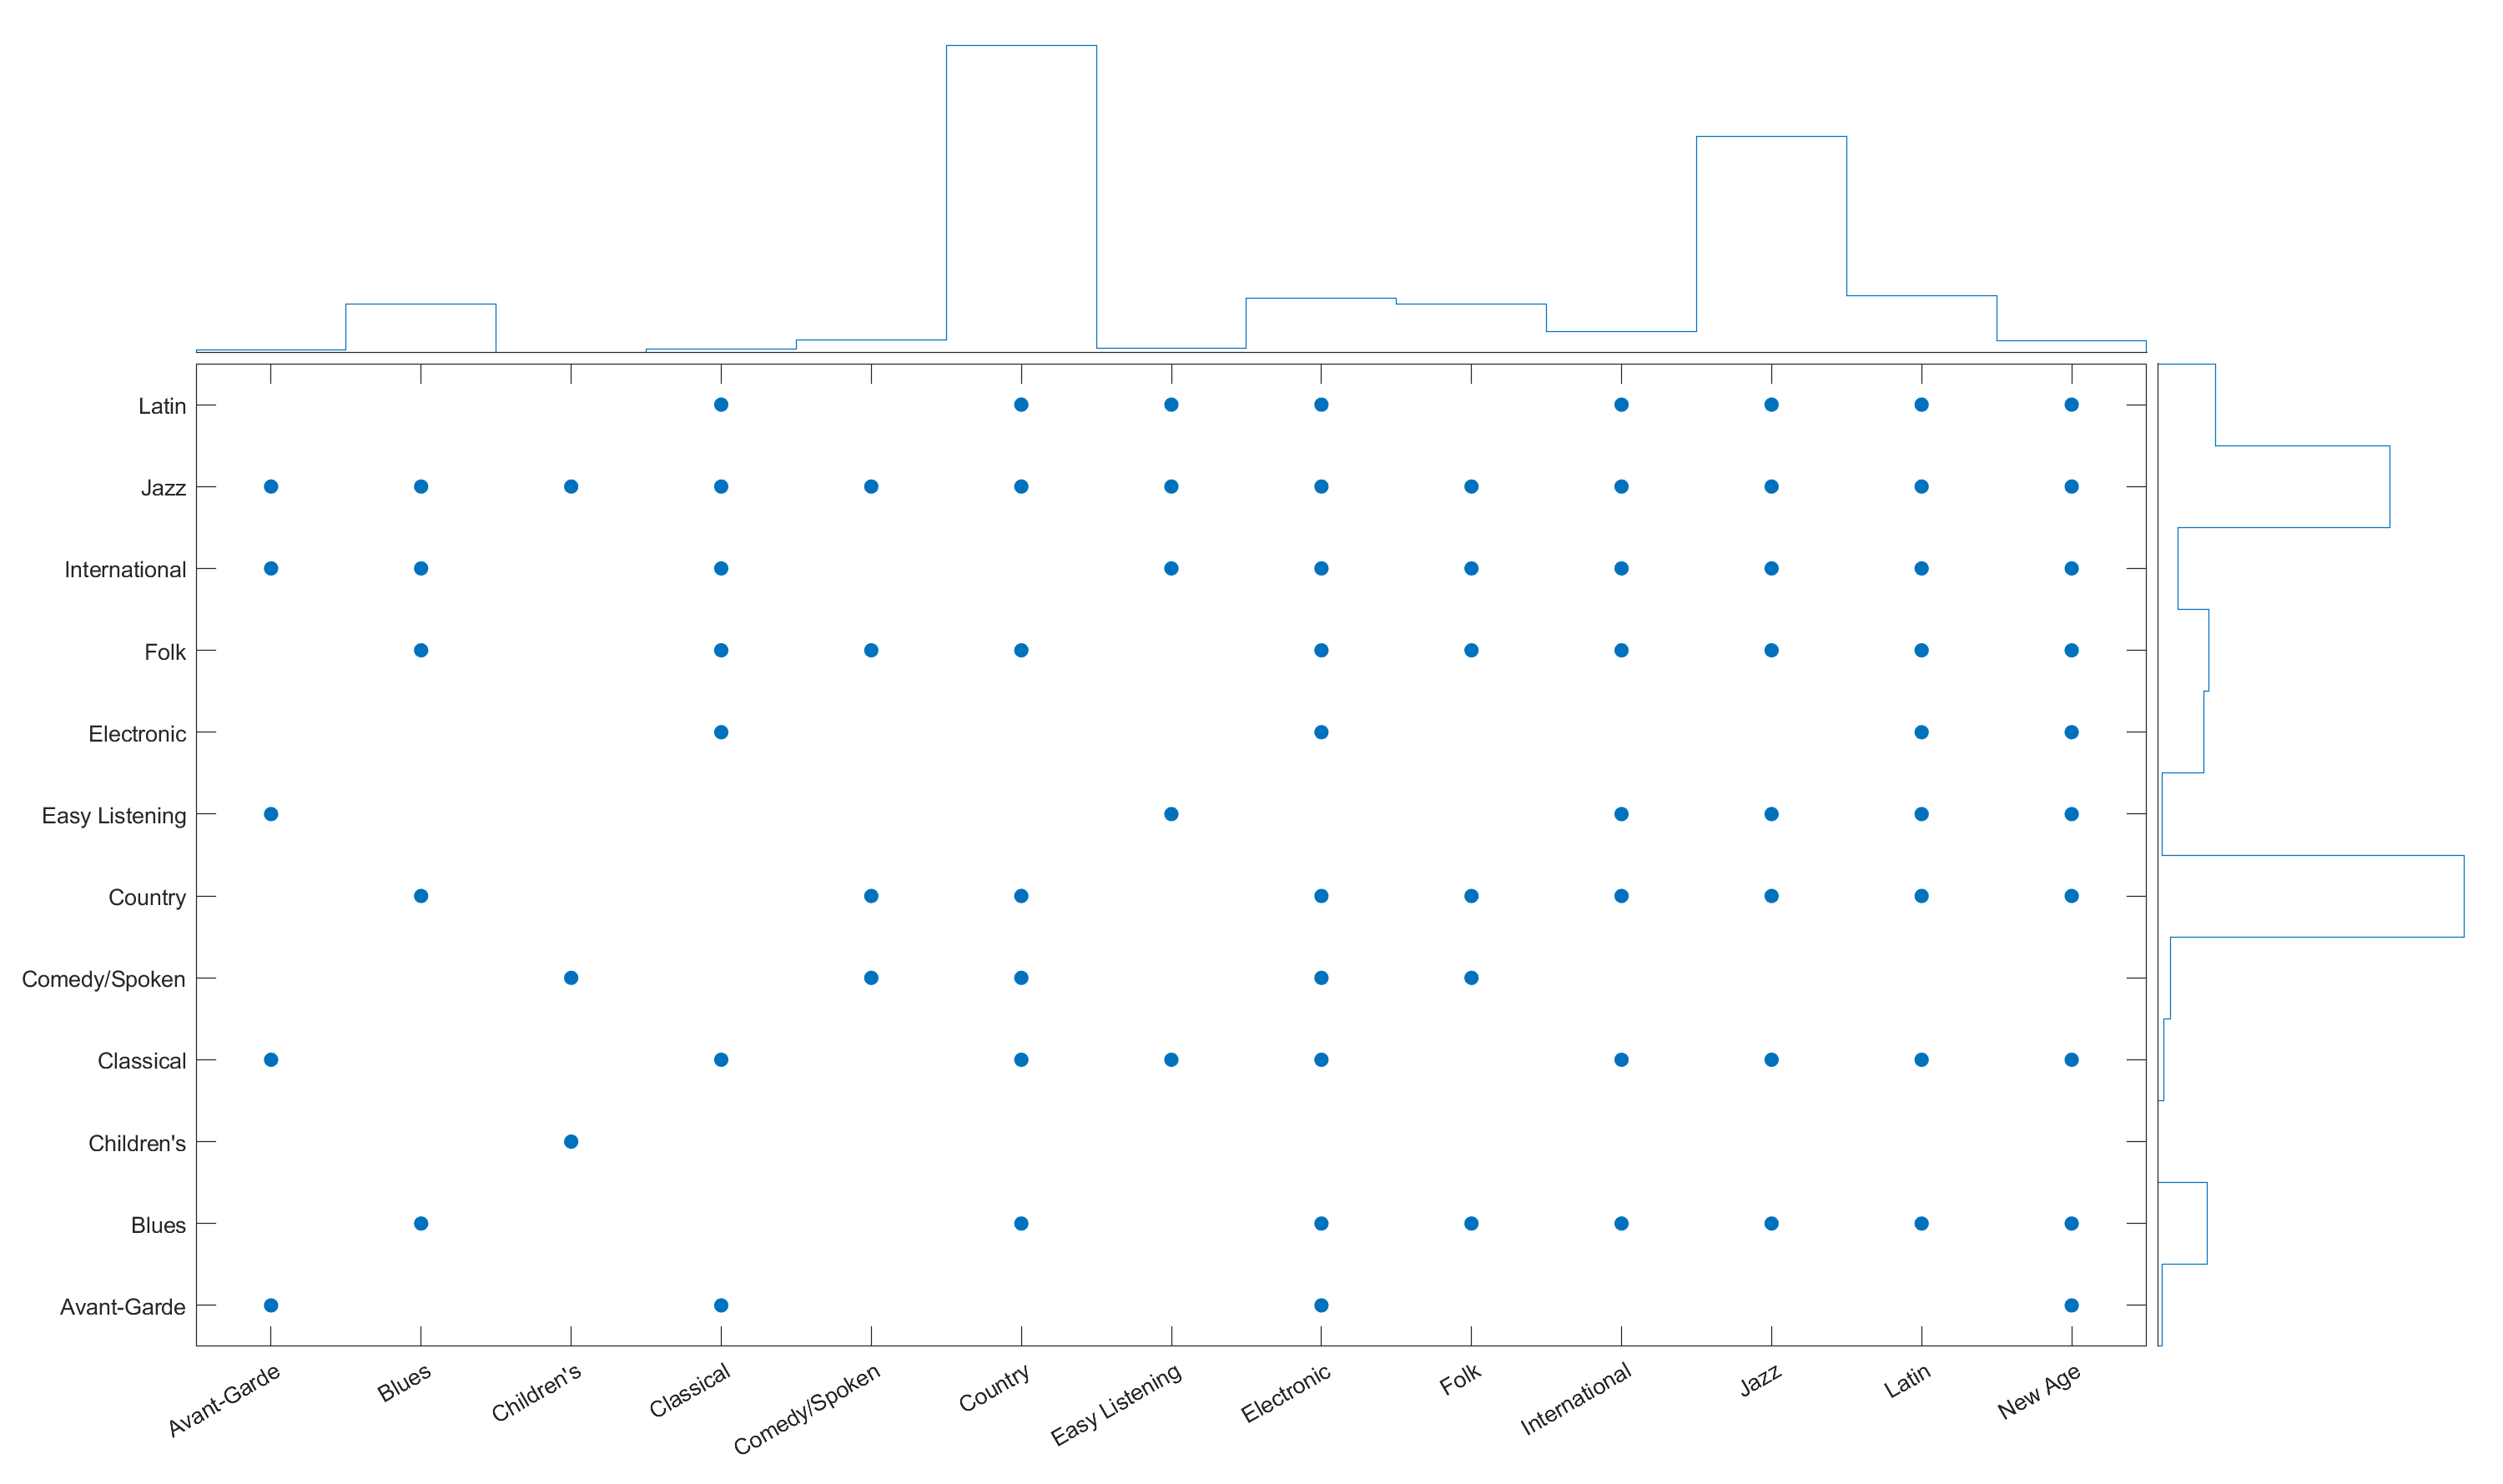
\includegraphics[scale=0.07]{Music14}\\
(Dot: Whether the link exists)\\
(Bar: The Duration of the Link)
\caption{Chart of Link Between Genres}
\end{wrapfigure}

After processing the provided data by wrapping the genre {\textit{unknown}} out, putting the index of various factors of musical work into calculation of {\textsc{cs}} among genres and making out the calculation the average of {\textsc{cs}} of the song of the same genre, we can gain access to the following chart, where similarity stay high in the red blocks and low in the green ones.
\\\\\\\
\begin{wrapfigure}{l}{0cm}
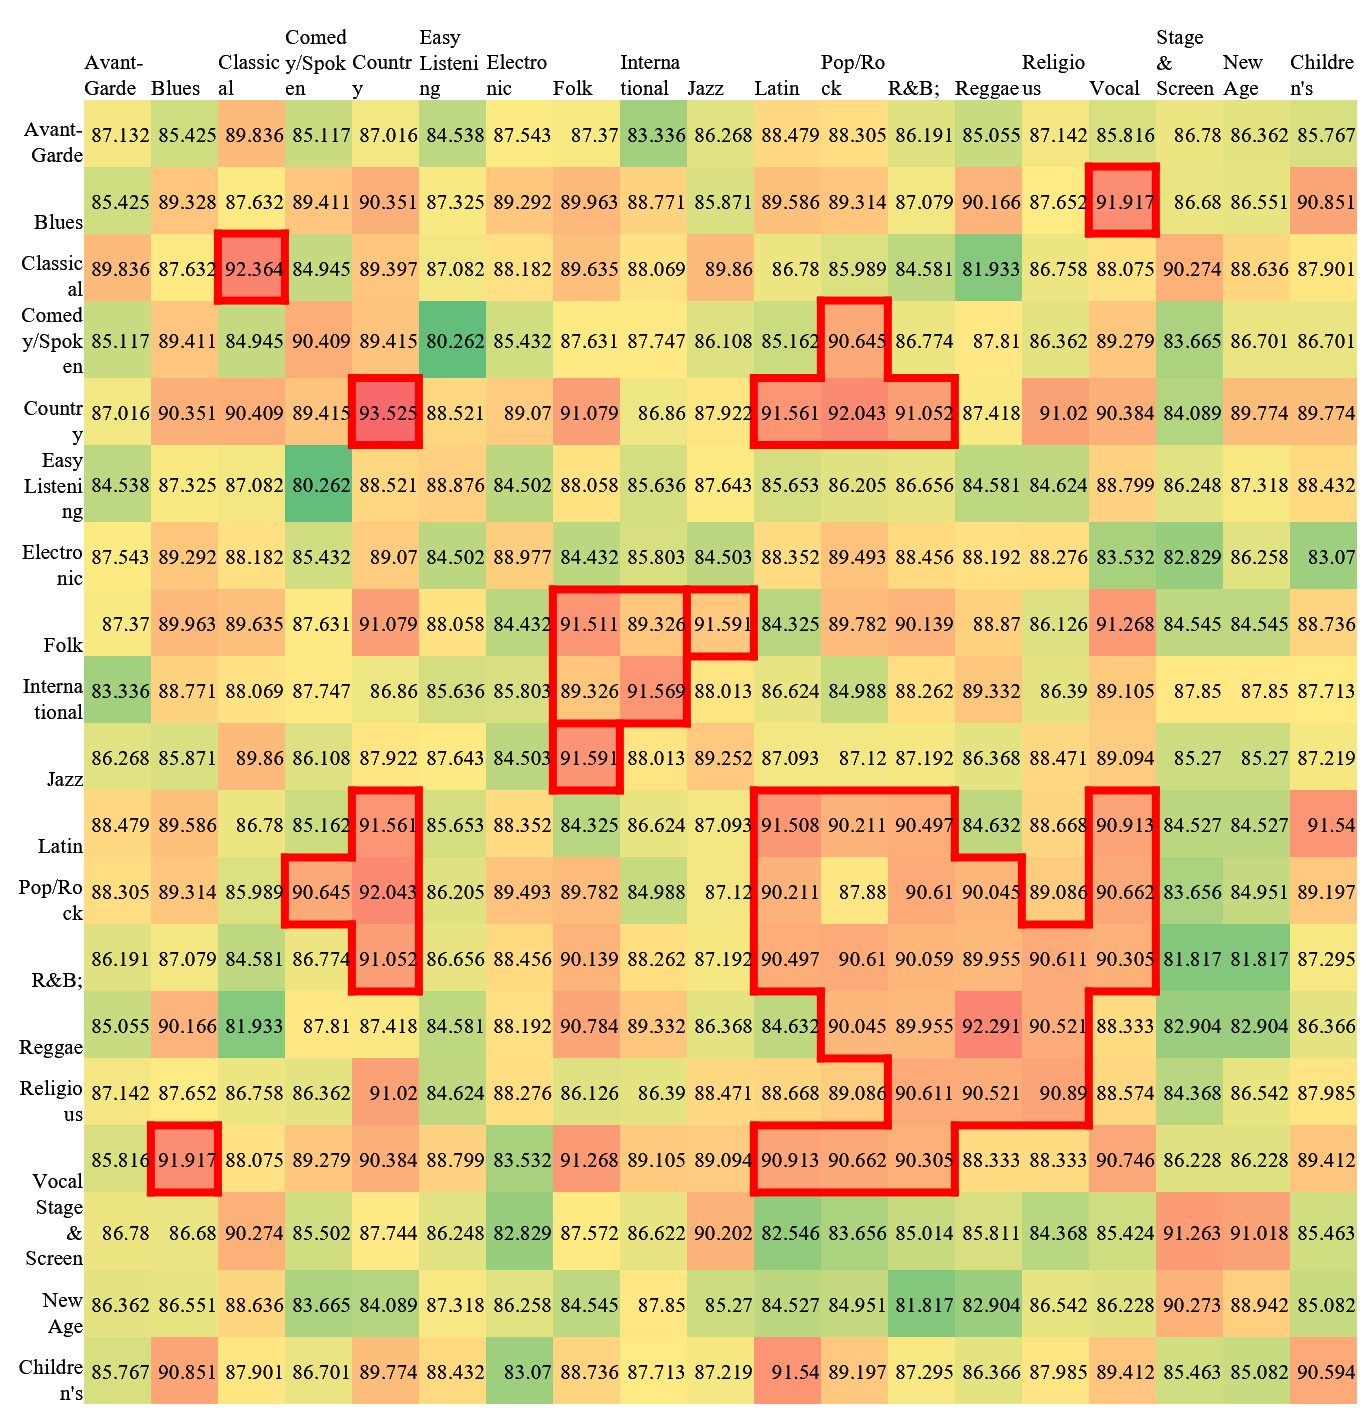
\includegraphics[scale=0.2]{Music8}	
\end{wrapfigure}

The figure shows that:
\begin{itemize}
	\item The genres {\textit{pop/rock, Latin, R\&B, reggae, religious}} and {\textit{vocal}} feature high similarity with each other, making the fact clear that the role they played during the development of music have been magnificent.
	\item It's not necessary that the works get the most of the influences from those of the same genres.
	\item Works of music may leave rare influence on others if they follow different paths of era or targets; But these influences can't be ignored.\\\\\\\\\\\\
\end{itemize}
\subsubsection{Discussion of Songs of Different Genres}
Our team solved the average of all the information of the works of the same genre and got the following bar chart after the process of standardization of all stats.
\begin{figure}[h]
	\centering
	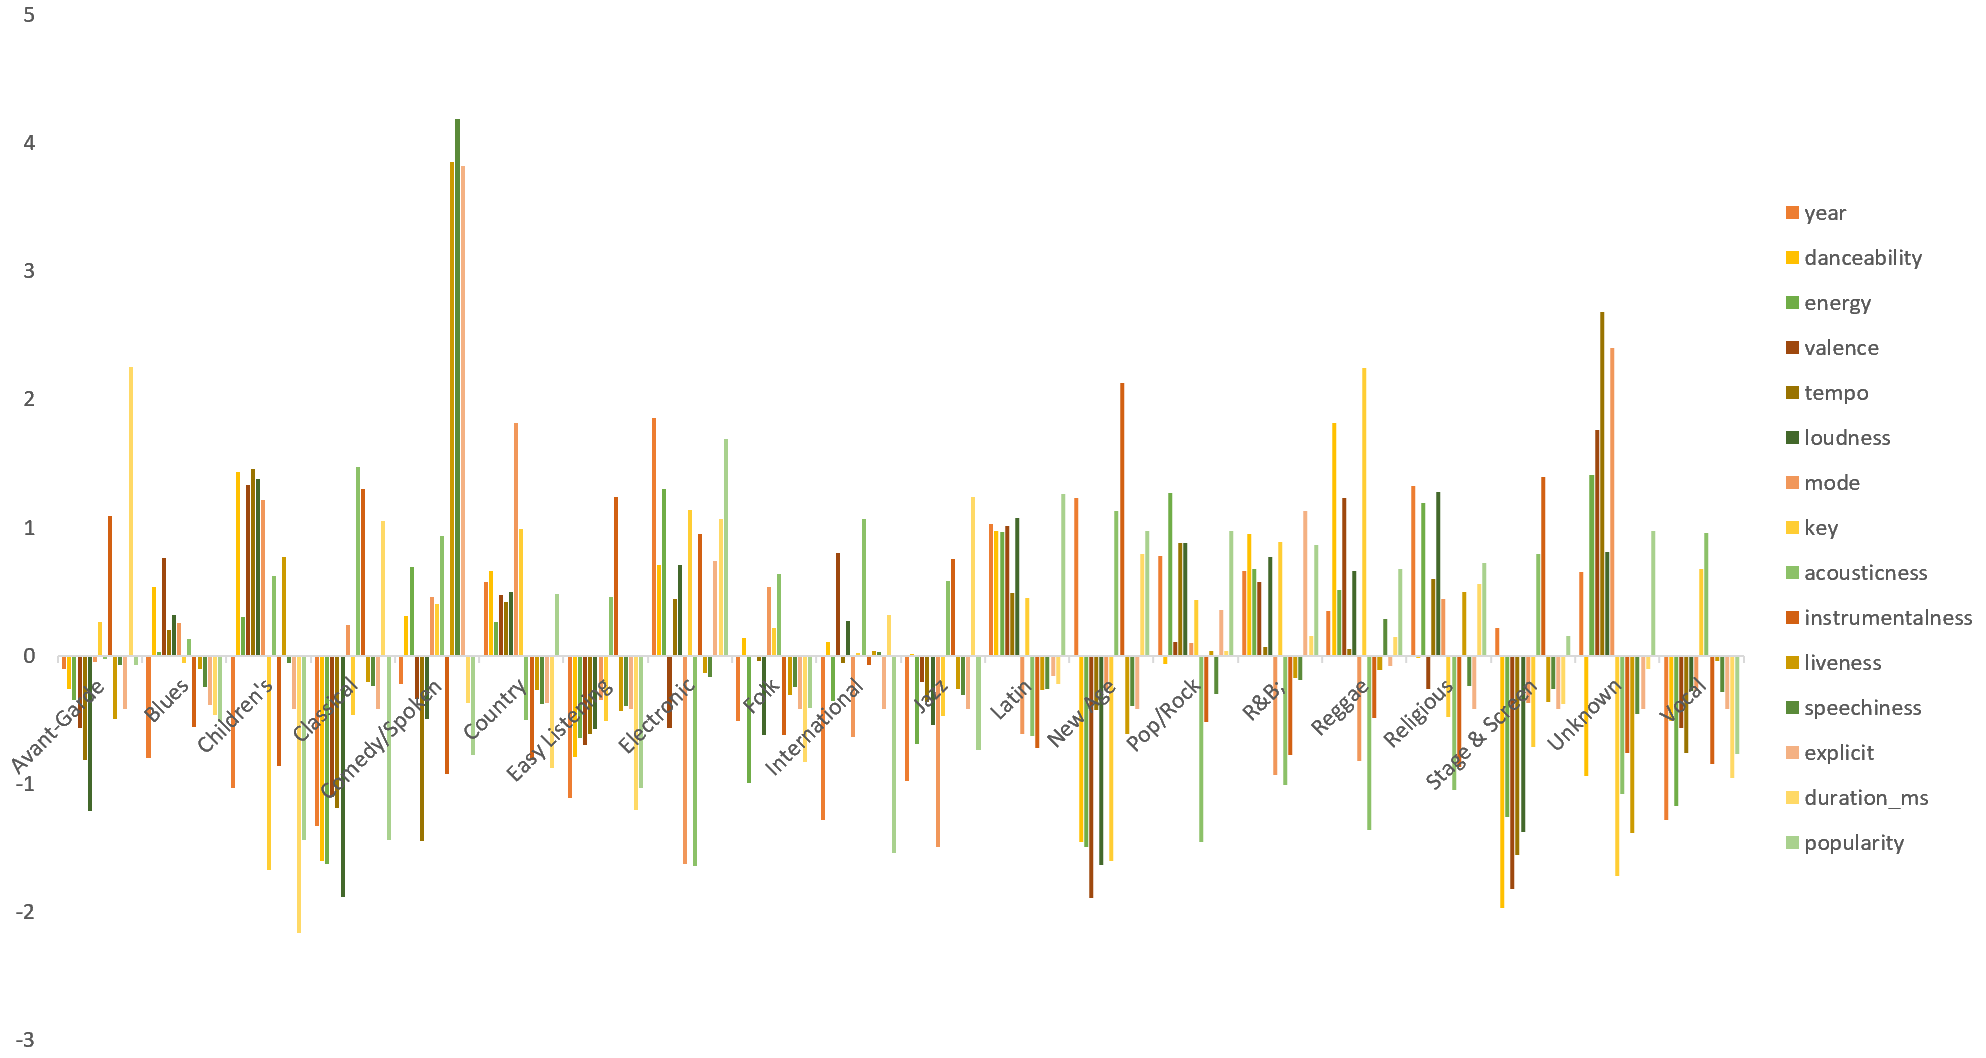
\includegraphics[scale=0.19]{Music10}
	\caption{Bar Chart of Characteristics' Info}
\end{figure}\\
The figure above indicates that:
\begin{itemize}
	\item {\textit{Classical international, Electronic}} and {\textit{Religious}} come into existence much later than others. The first one can be categorized as a classics, while the latter 2 can be regarded as modern music.
	\item {\textit{Reggae}} and {\textit{Childen's}} stand out when it comes to the best dance-suited tracks. They possess optimistic tracks, the ones which {\textit{New Age, Stage \& Screen}} and {\textit{Comedy/Spoken}} do not feature, as well.
	\item {\textit{Electronic}} and {\textit{Pop/Rock}} feature the most energetic tracks while the {\textit{New Age}} and {\textit{Classical}} stand the opposite.
	\item {\textit{Pop/Rock}} and {\textit{Children's}} feature the most strong tempo which {\textit{Stage \& Screen}} don't possess.
	\item {\textit{Children's, Religious}} and {\textit{Latin}} feature loudness.
	\item {\textit{Reggae}} and {\textit{Electronic}} are characterized with high pitch while the genre {\textit{Children's}} feature low pitch.
	\item When it comes to the percentage of instrumentalness, {\textit{New Age}} and {\textit{Stage \& Screen}} stand out to be the highest, while {\textit{Classical New Age}} turn out the lowest. More elements of electronics, namely, take place in {\textit{Electronics}}.
	\item {\textit{Electronics, Latin}} and {\textit{New Age}} enjoy top popularity, while the scene of {\textit{Comedy/Spoken}} and {\textit{Children's}} may be hot when covered live.
\end{itemize}
\subsection{Analyzing Turning Points in the Development of Music}
The analysis is purposed at solving \textbf{Problem 5} in the restatements.\\[2ex]
After the factors analysis conducted in {\textbf{4.1.3}} with the help of using the parameters in the file {\textit{data\_by\_year.csv}}, we can get the value of $F$ in the equation (3).
Our team have to conduct a process of standardization for $F$ due to the large amount of it, having succeeded in getting the new parameter $F^{'}$. The line chart of $F^{'}$ in terms of year is as follows.
\begin{figure}[h]
\centering
	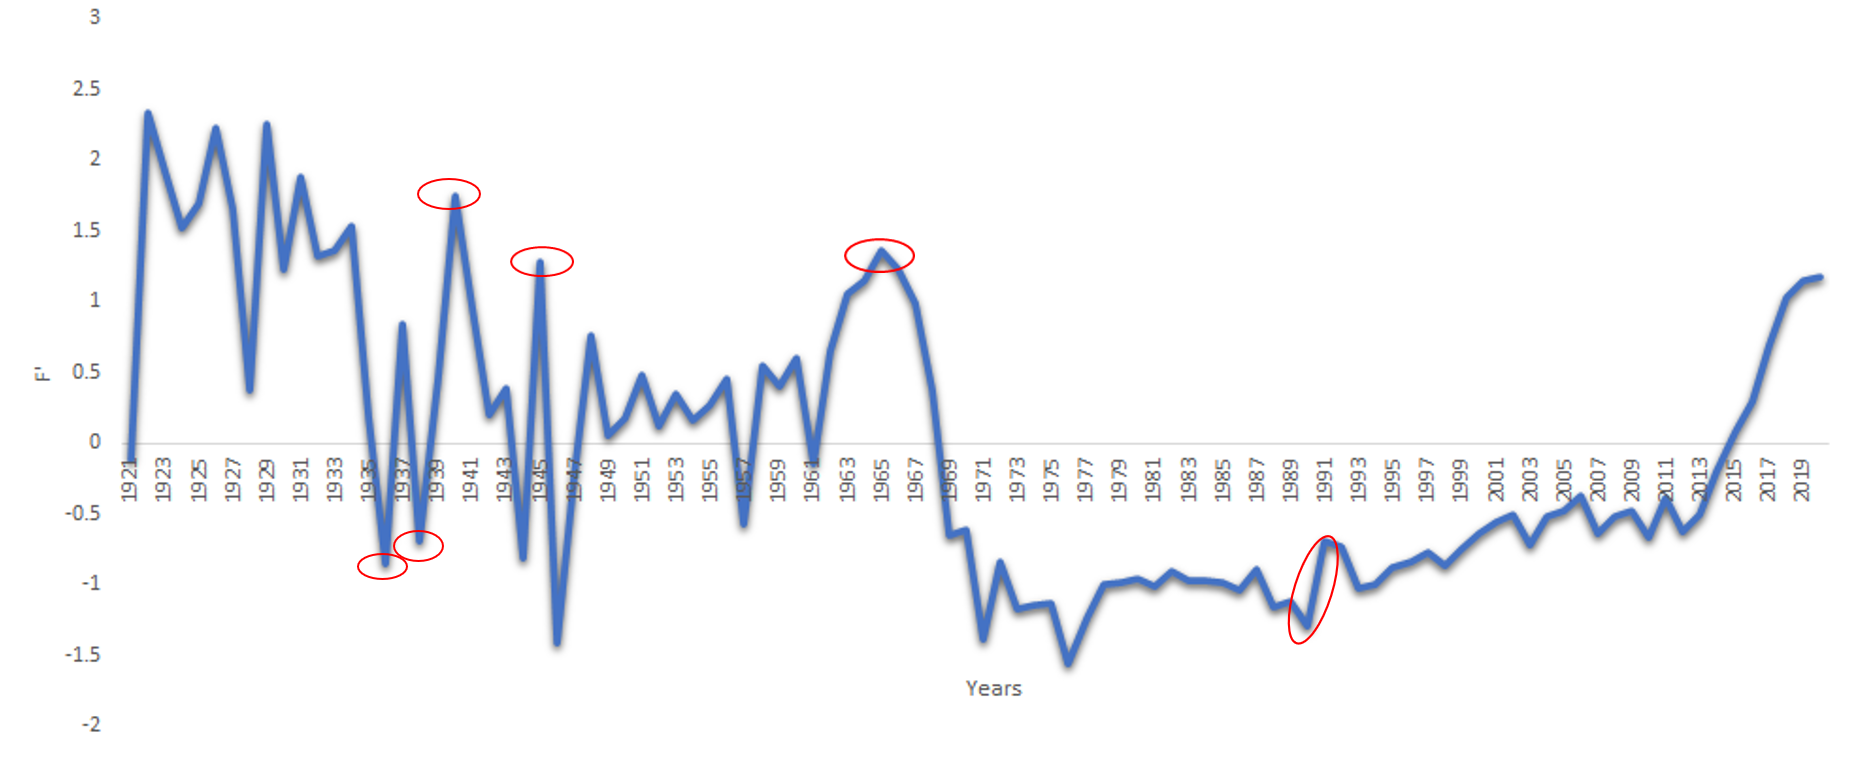
\includegraphics[scale=0.13]{Music11}
	\caption{Line Chart Featuring $Y_i$ and $F^{'}$}
\end{figure}\\[2ex]
The figure indicates that the development of music, as is illustrated in the circle-marked point, have experienced great shifts in 1936, 1938, 1945 and 1965.\\[2ex]
Having taken the years into account, we found out the revolutionary musicians in the 1940s and 1960s by depicting the networks respectively.
\begin{figure}[htbp]
\centering
\begin{subfigure}[The 1940s]{
	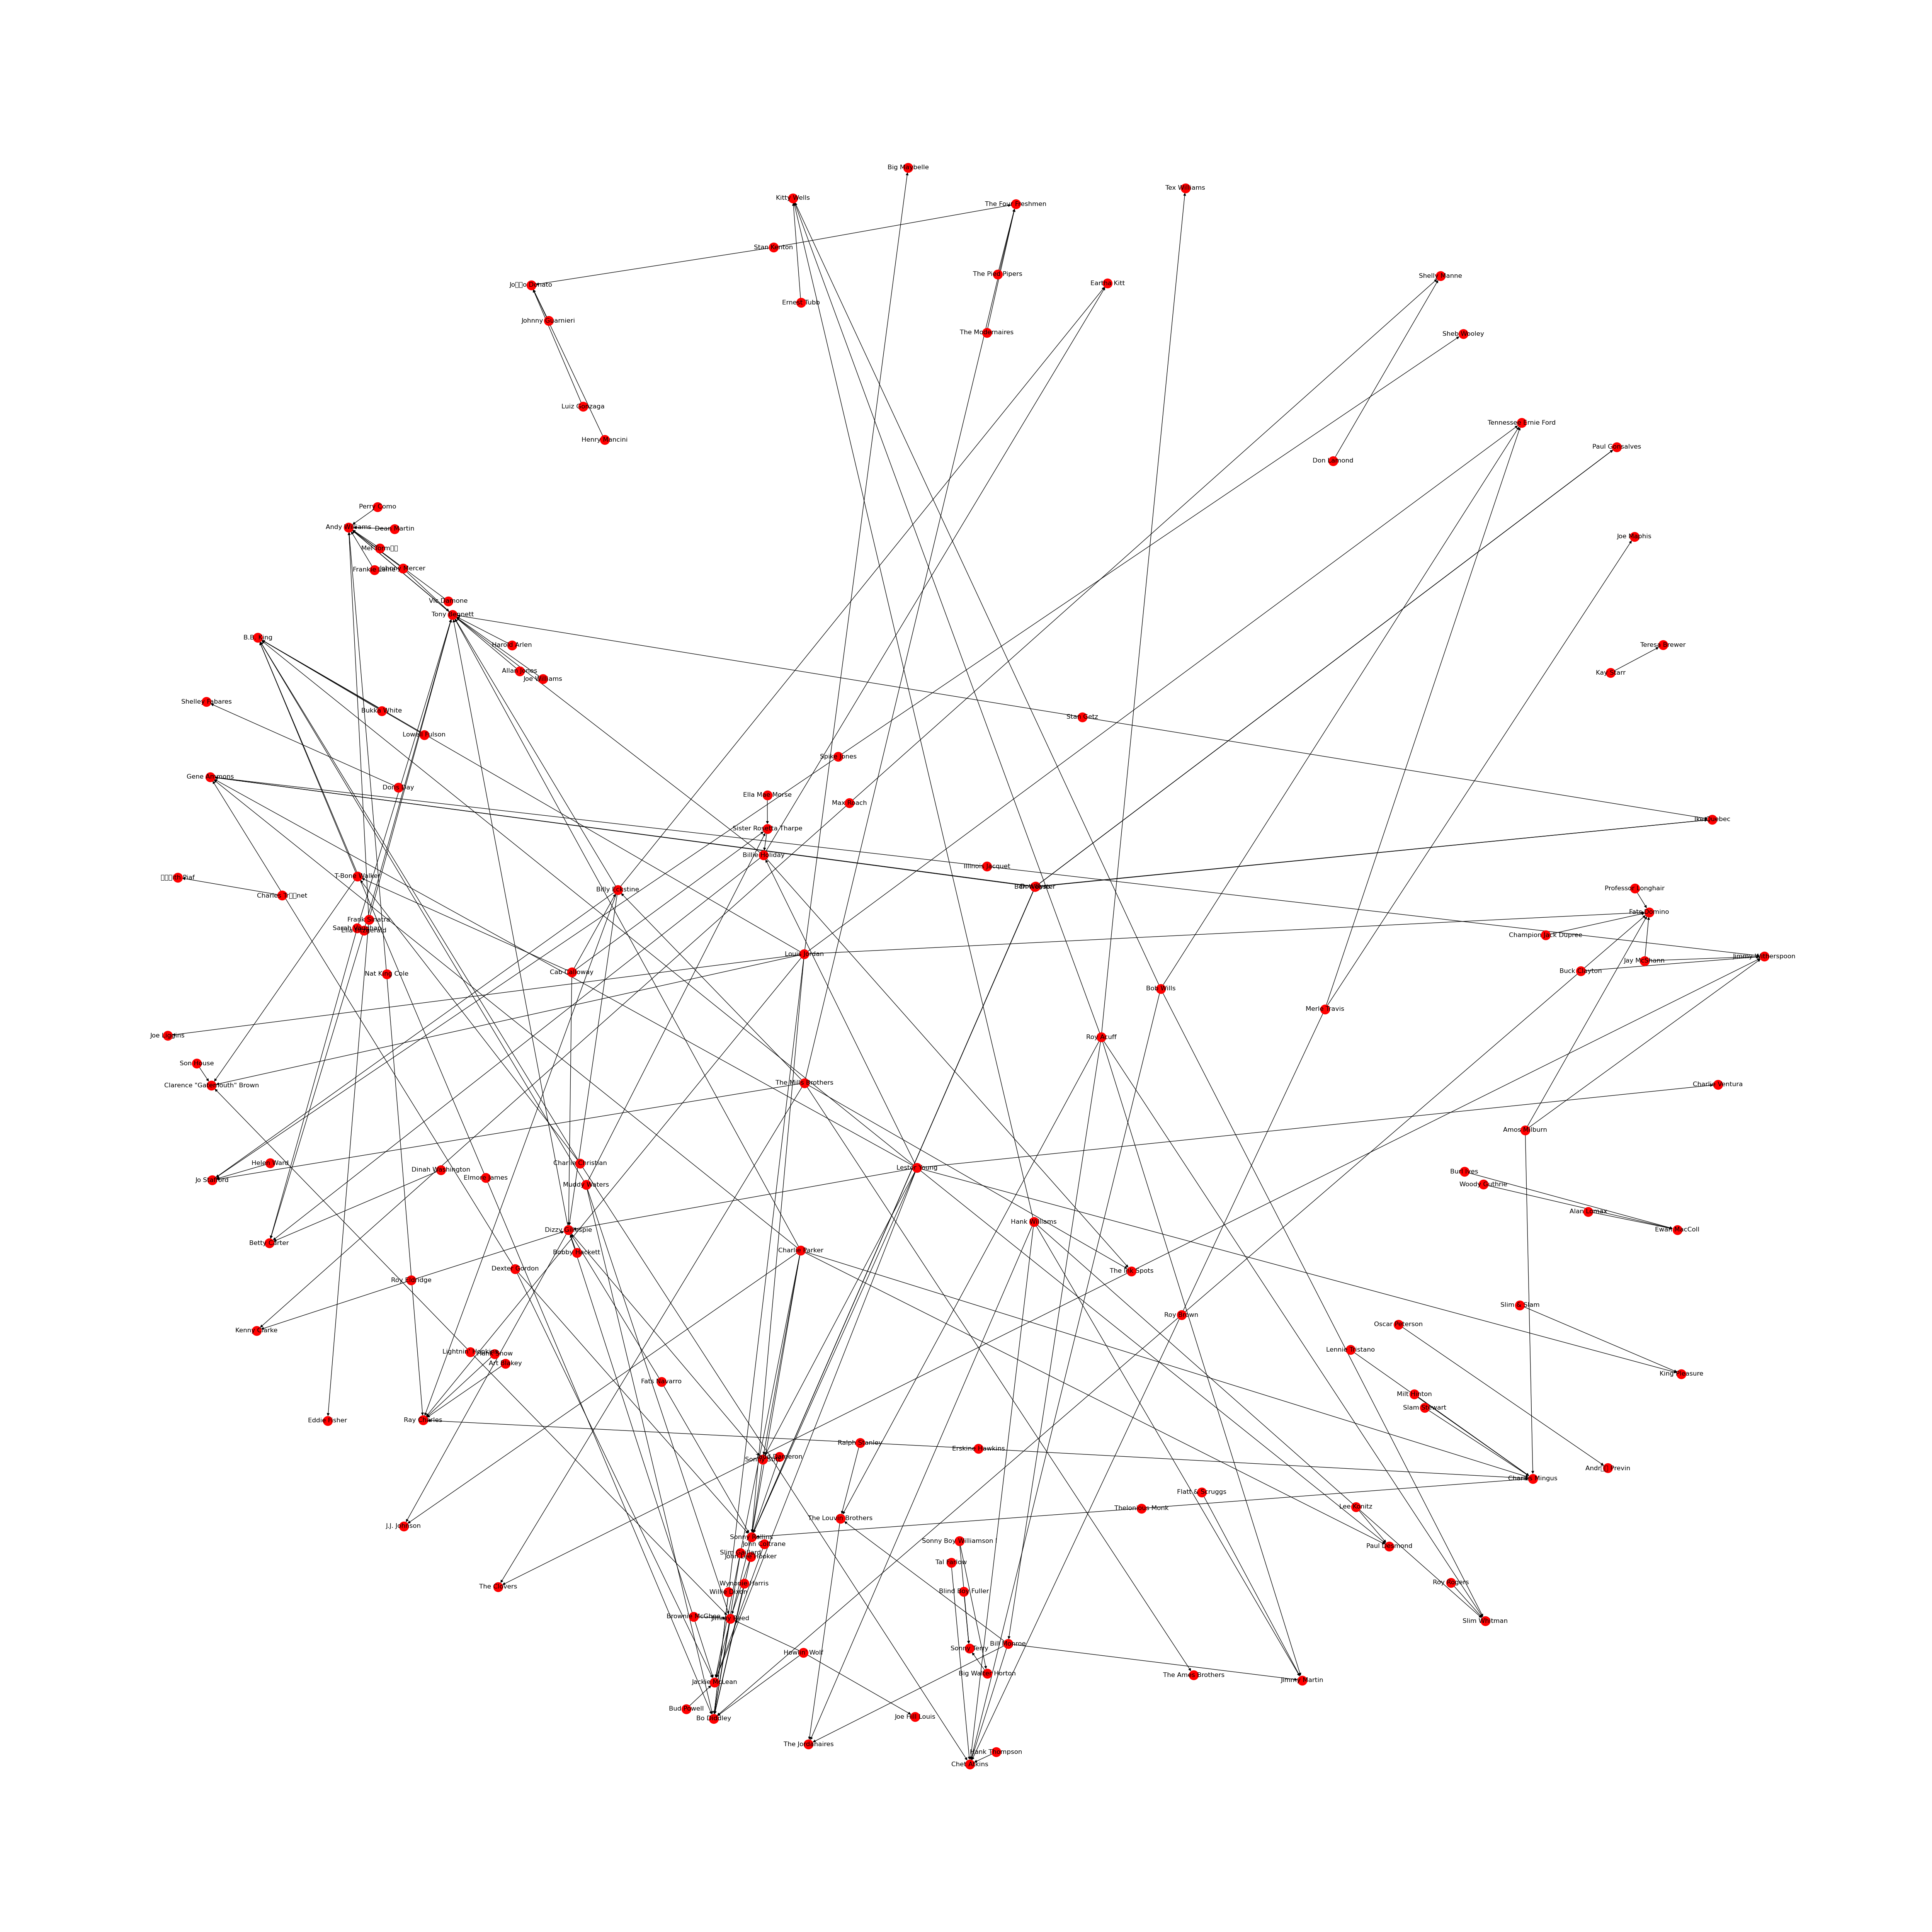
\includegraphics[scale=0.053]{Music12}
}
\end{subfigure}
\hspace{1.8cm}
\begin{subfigure}[The 1960s]
{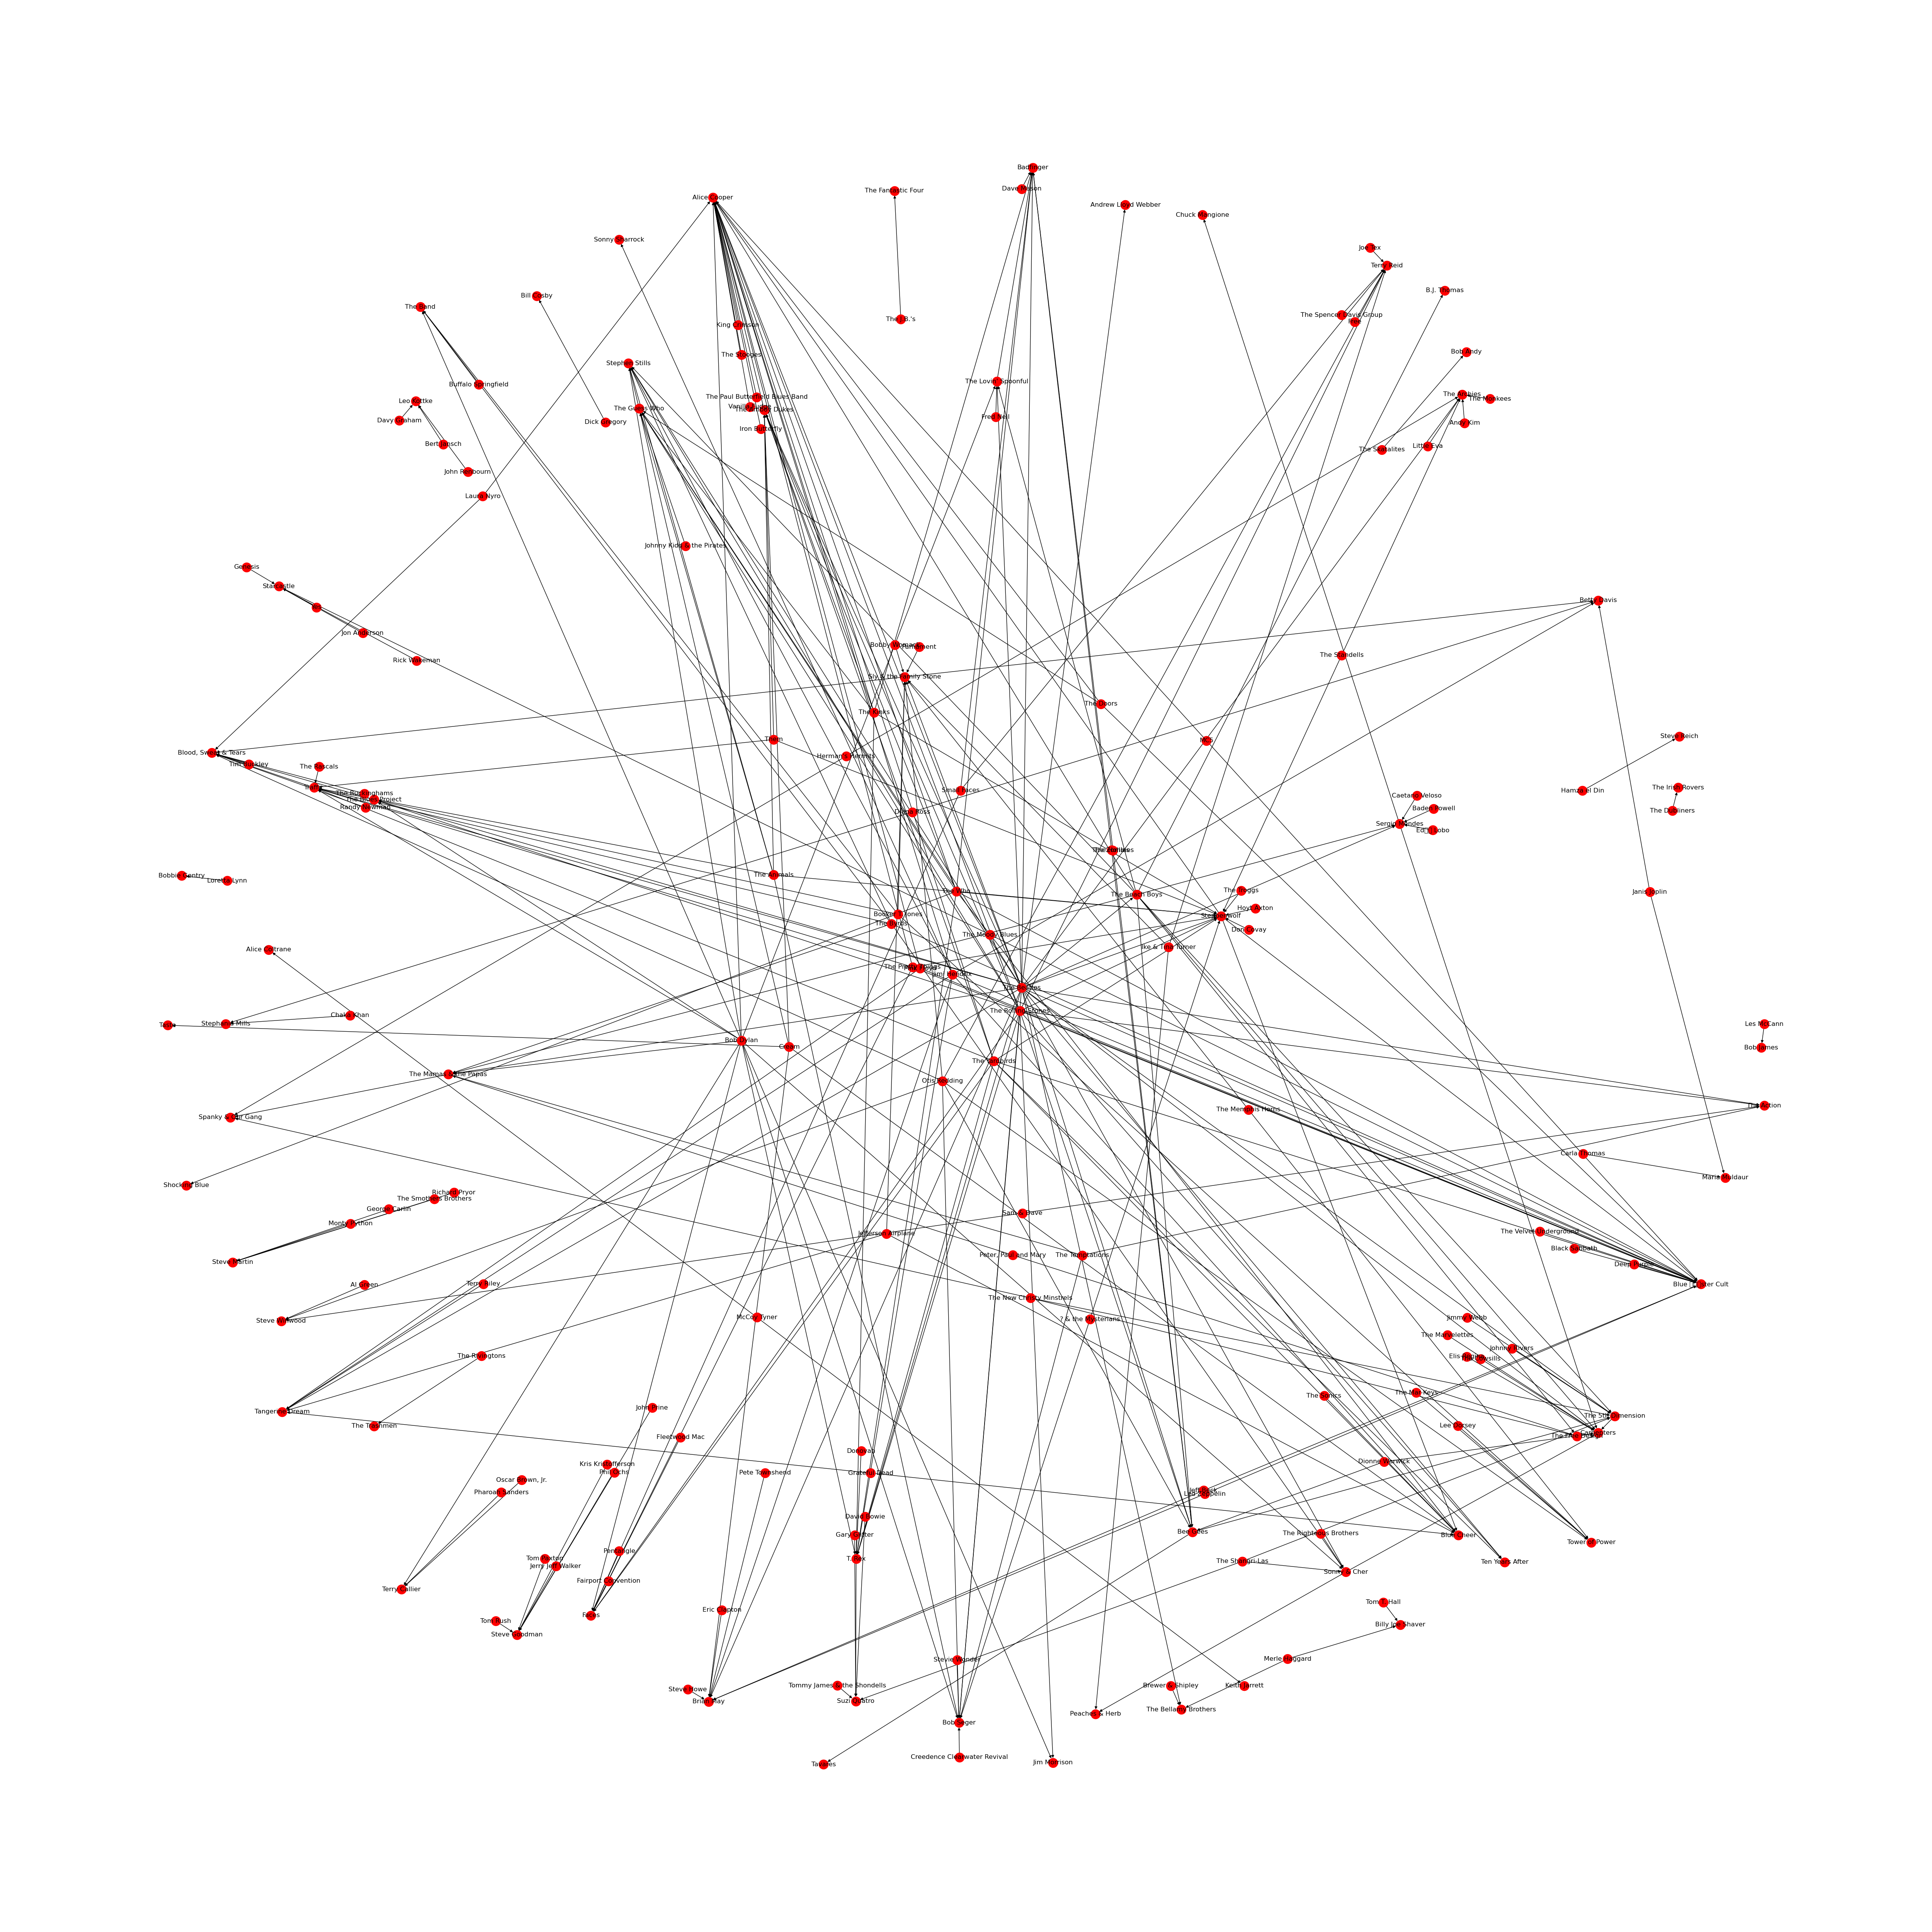
\includegraphics[scale=0.053]{Music13}}	
\end{subfigure}
\caption{Networks in the 1940s \& the 1960s}
\end{figure}\\[2ex]
Using the figure above, we can safely say that \textit{vocal} and \textit{jazz} enjoyed popularity in the 1940s, the era when Charlie Parker, John Coltrane and Lester Young leave the deepest influence on the atmosphere. \textit{Pop/Rock}, as is reported in the network, were given birth to by the music of the mainstream. \textit{Blue, R\&B} also got influenced by \textit{jazz and country}.\\[2ex]
Similarly, \textit{Pop/Rock} turn mainstream in the 1960s with over a half of the artists enjoying it. \textit{Blue, jazz} and \textit{R\&B} also gained widespread applause in the society, making great impact on \textit{Stage \& Screen Reggae} and resulting in the birth of \textit{Reggae}. The network indicates that The Beatles, Alice Cooper, Paul weller and Soundgarden turned the most popular band or musical individuals.\\[2ex]
In short, the charts above displays the fact that \textbf{great shifts can be partly attributed to the existence of \textit{Pop/Rock} in the 1940s and \textit{Reggae} in the 1960s.}
\subsection{Analyzing Development of Music Over Time}
This model is a solution to \textbf{Problem 4} in the restatements. Our team solve this problem by analyzing with angles of artists and genres respectively.
\subsubsection{Sub-Model for Analyzing the Development of Artists Over Time}
According to the analysis of stats, we succeeded in finding that when it comes to followers of one artist, over half of the followers will create music of the same genre with the influencer's. For the exceptions of the musicians above, however, their compositions of other genres may feature high similarity with the works of their influencers. \textit{Rehab}, an \textit{R\&B} work, and \textit{Amateur (Rock Me Amadeus)}, a \textit{Latin} work, feature the incredible similarity of 99\% with each other. Other compositions of these exceptions play a great role in the phase of innovation. The Beatles once got affected by Slim Whitman, a \textit{Country} musician, King Curtis and Barrett Strong, \textit{R\&B} musicians. It was influences from those artists that give rise to the band's widespread influence and its high popularity. As a result, \textbf{the influencers actually affect the music created by the followers.}\\[2ex]
The researches conducted in \textbf{4.1} have told us that the indicators bringing the strong relationship with popularity are \textbf{energy, loudness and acoustics}. As a result, we're firmly convinced that these 3 parameters \textbf{plays the strongest pushing role for the influence on the followers} as well. To prove the conclusion we made, we studied the influencers and followers of Aice Cooper, the origin of \textit{Hard Rock, Heavy Metal} and \textit{Pop/Rock}, of which the result is shown below.
\begin{figure}[h]
\centering
	\begin{subfigure}[Followers of Alice Cooper]
		{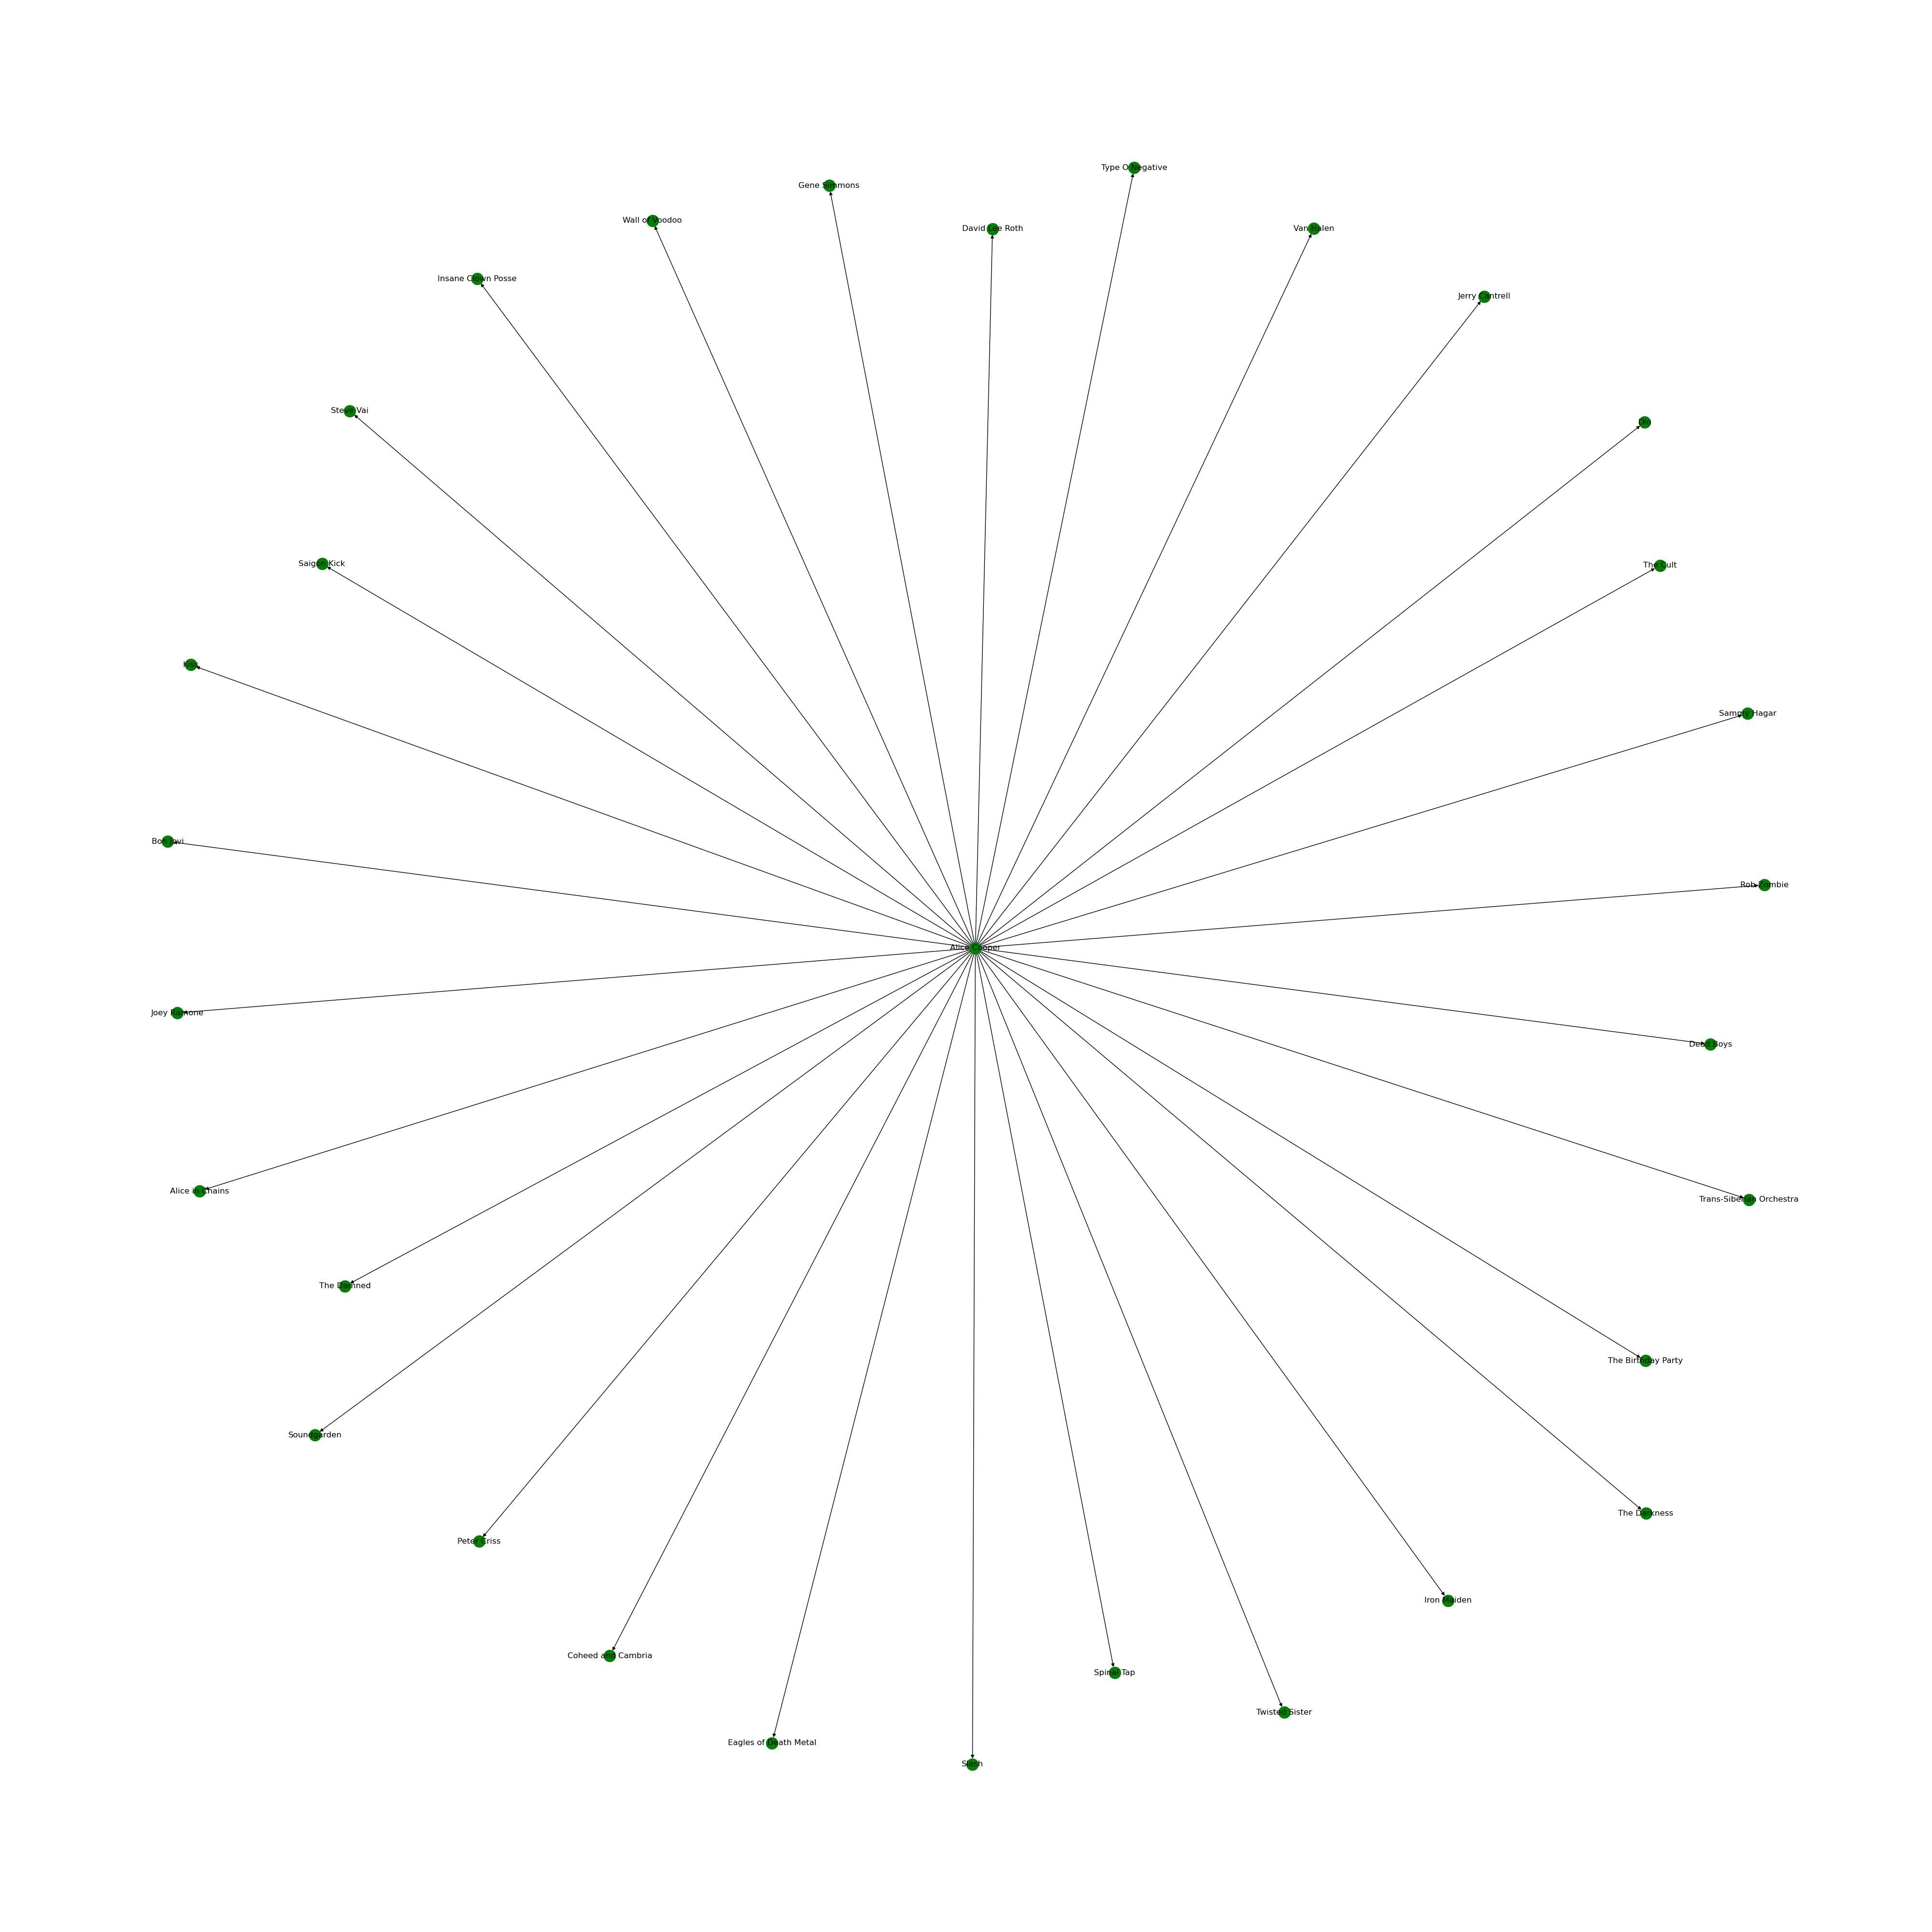
\includegraphics[scale=0.054]{Music18}}
	\end{subfigure}
	\hspace{1.5cm}
	\begin{subfigure}[Influencers of Alice Cooper]
		{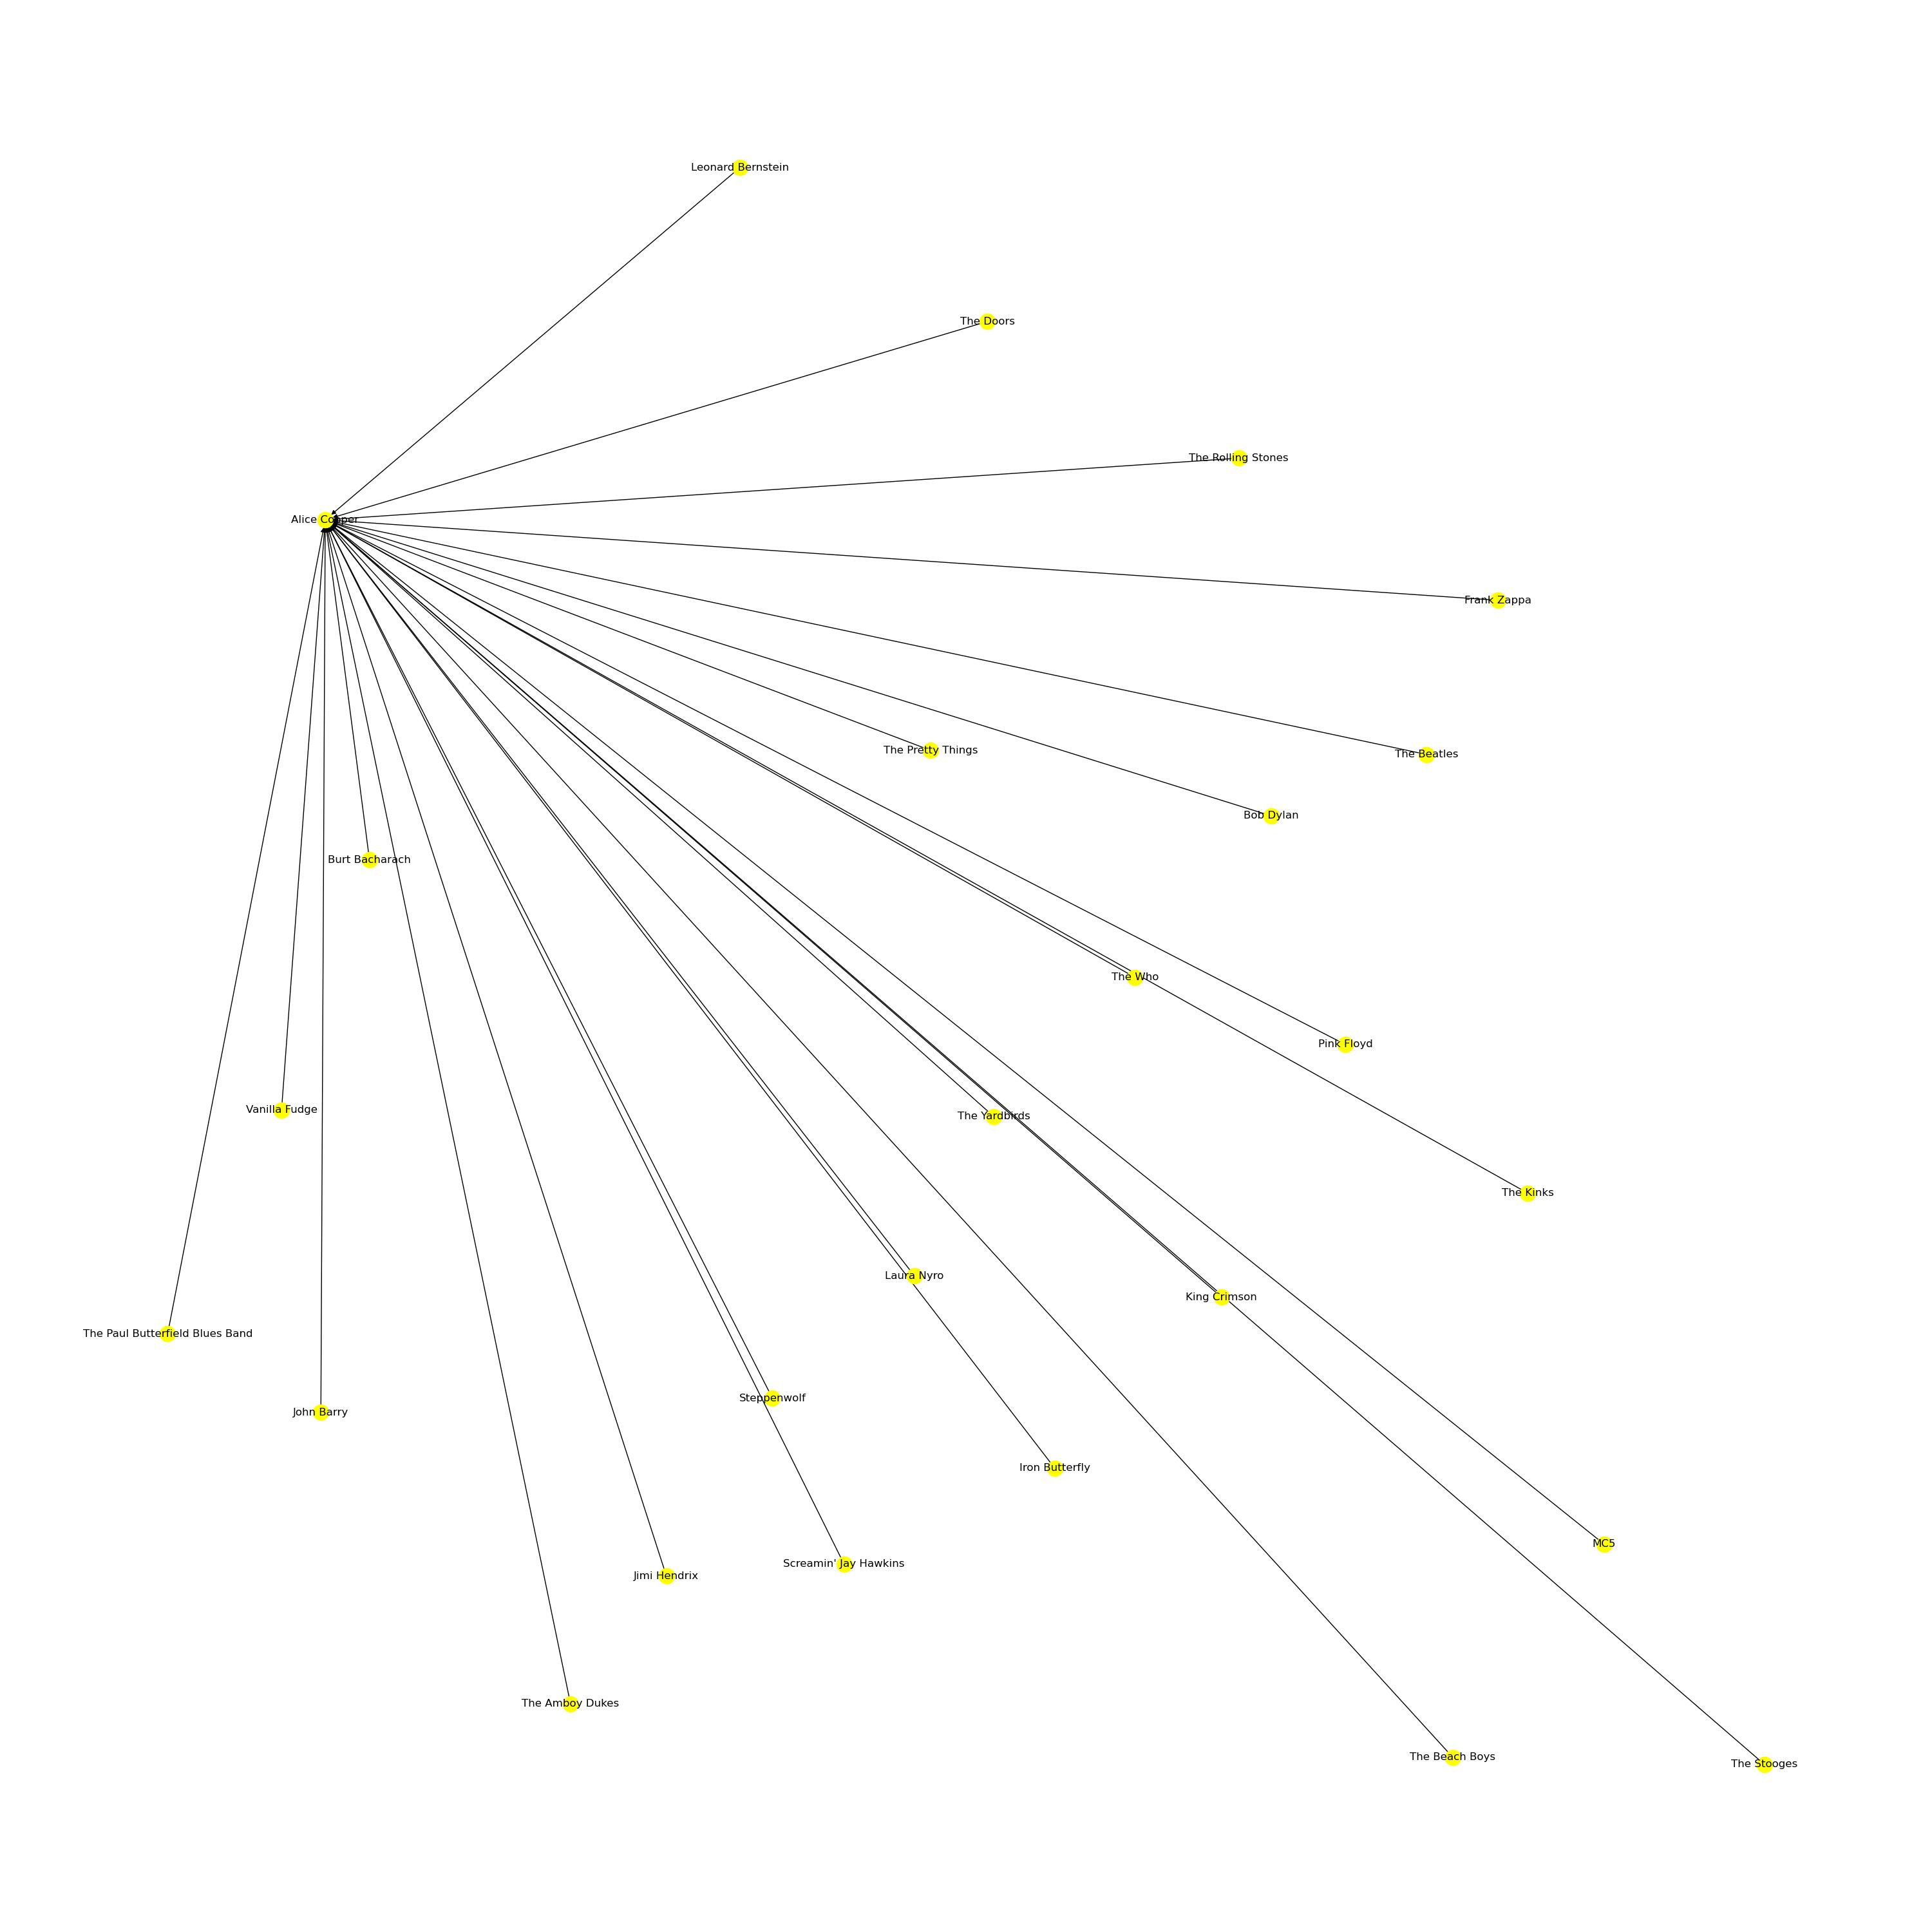
\includegraphics[scale=0.072]{Music17}}
	\end{subfigure}
\end{figure}\\
Our team then analyzed key indicators of random 10 artists in the network and standardized the stats and depicted the radar charts below.
\begin{figure}[h]
\centering
	\begin{subfigure}[]
		{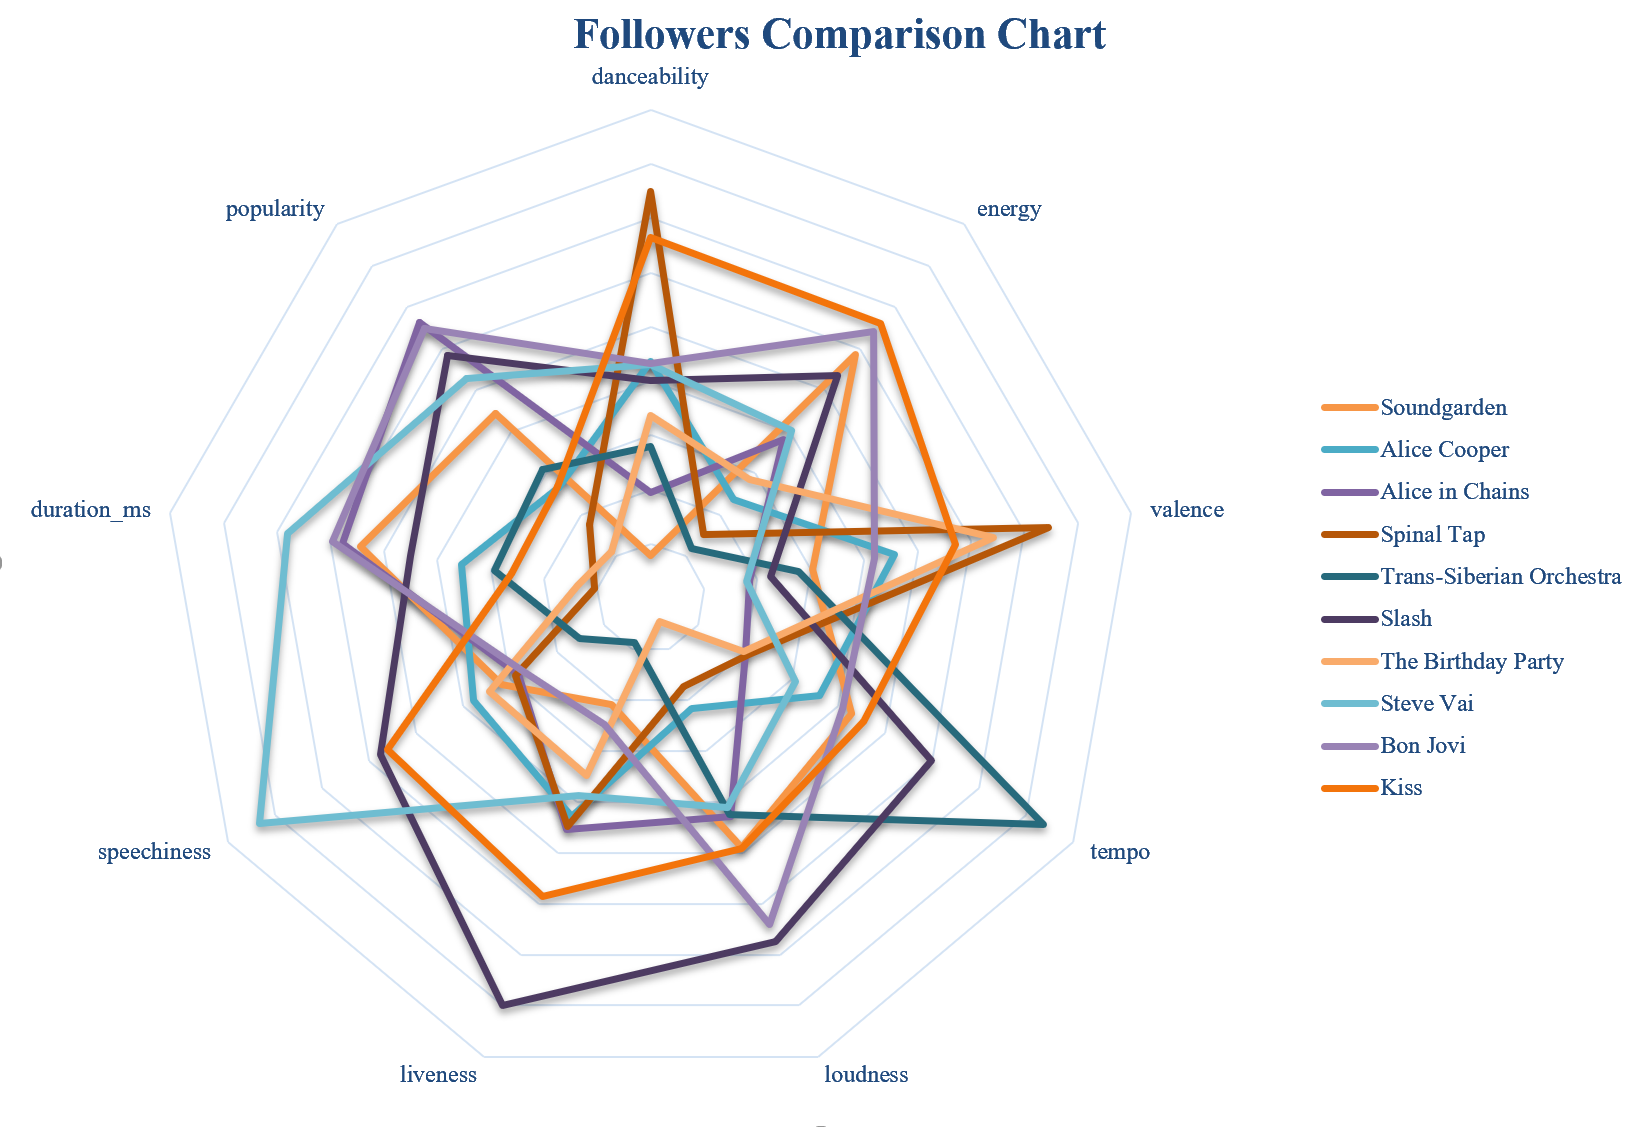
\includegraphics[scale=0.1]{Music15}}
	\end{subfigure}
	\hspace{0.5cm}
	\begin{subfigure}[]
		{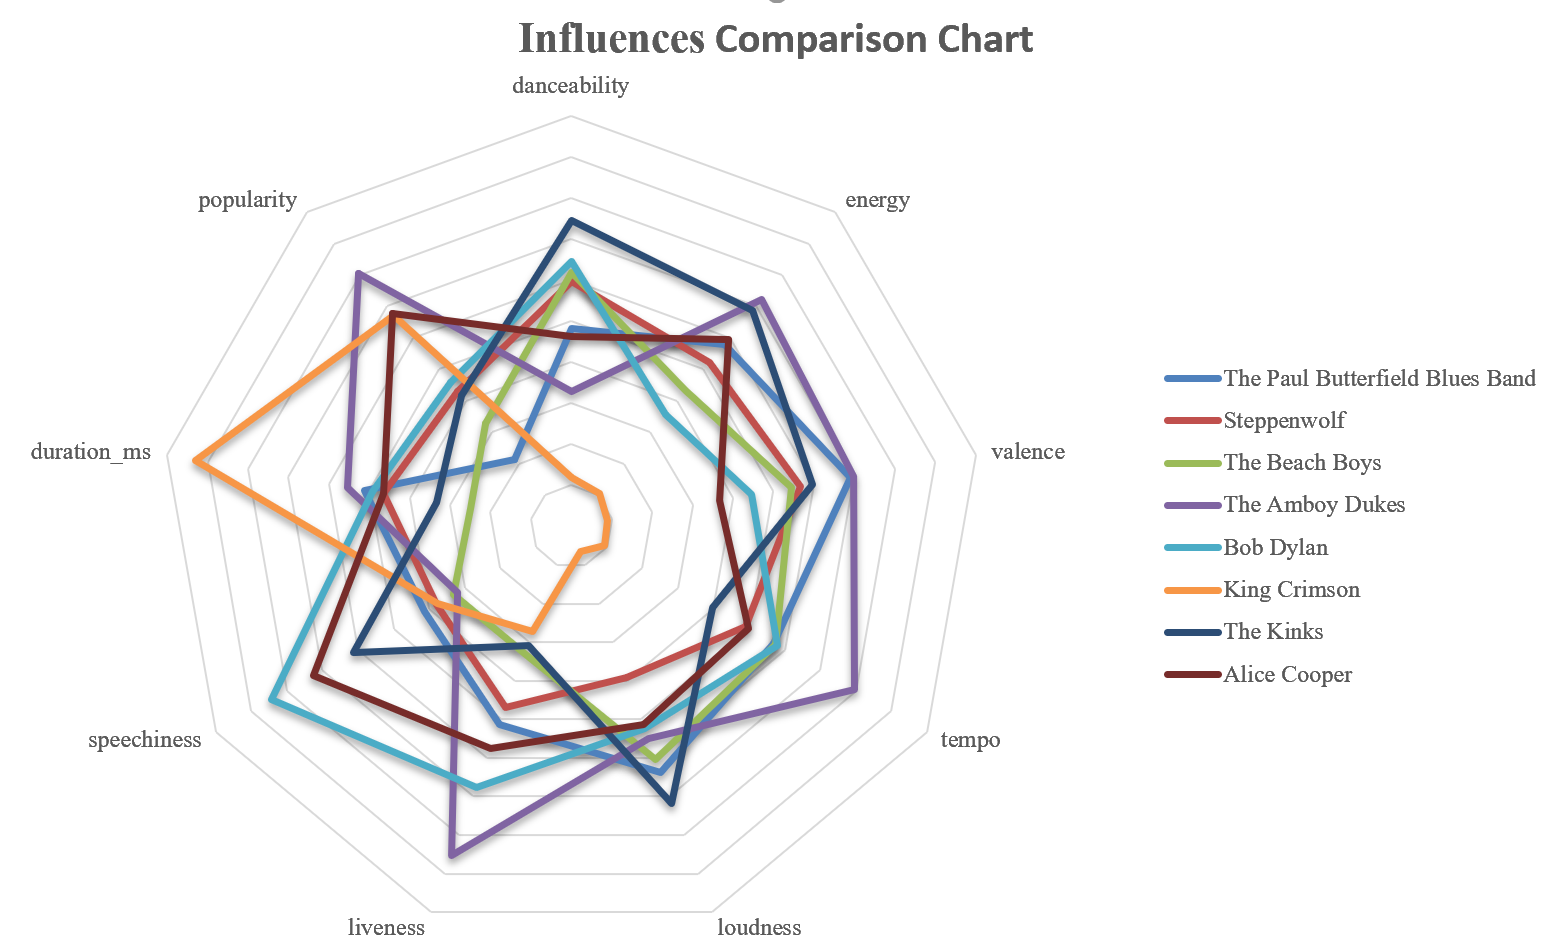
\includegraphics[scale=0.12]{Music16}}	
	\end{subfigure}
\caption{Network and Radar Charts of Followers and Influencers}
\end{figure}\\
As is illustrated, loudness and danceability are quite similar. In another word, Alice Cooper succeeded in absorbing these 2 factors into his work, thus gaining higher popularity than the former giants on their shoulders. Followers of Alice Cooper feature high similarities in valence, danceability and energy, but only 2 of them gained more popularity than their origins, indicating A.C.'s high musical achievements.\\[2ex]
In short, \bfseries{danceability and energy are more contagious than others. Meanwhile, the cliché \textit{better navigators, better destinations} is still making sense.}}
\subsubsection{Sub-Model for Analyzing Development in Genres Over Time}
The rock carved with the name of the genres will stand the tests of the scrubbing of the history. The characteristics of works of one genre may change according to the influences from other genres. Influences may occur among artists of the same genre; even some contagious factors of works from different genres may get inherited by their followers and the influences, if piled up, may bring up the storm of reforms. The increment may also increase as the number of artists within the genre increases. This effect may bring shifts on characteristics of some genres and the birth of new genres. The coming-up research is focused on the development of genres over time.\\
\begin{wrapfigure}{l}{0cm}
	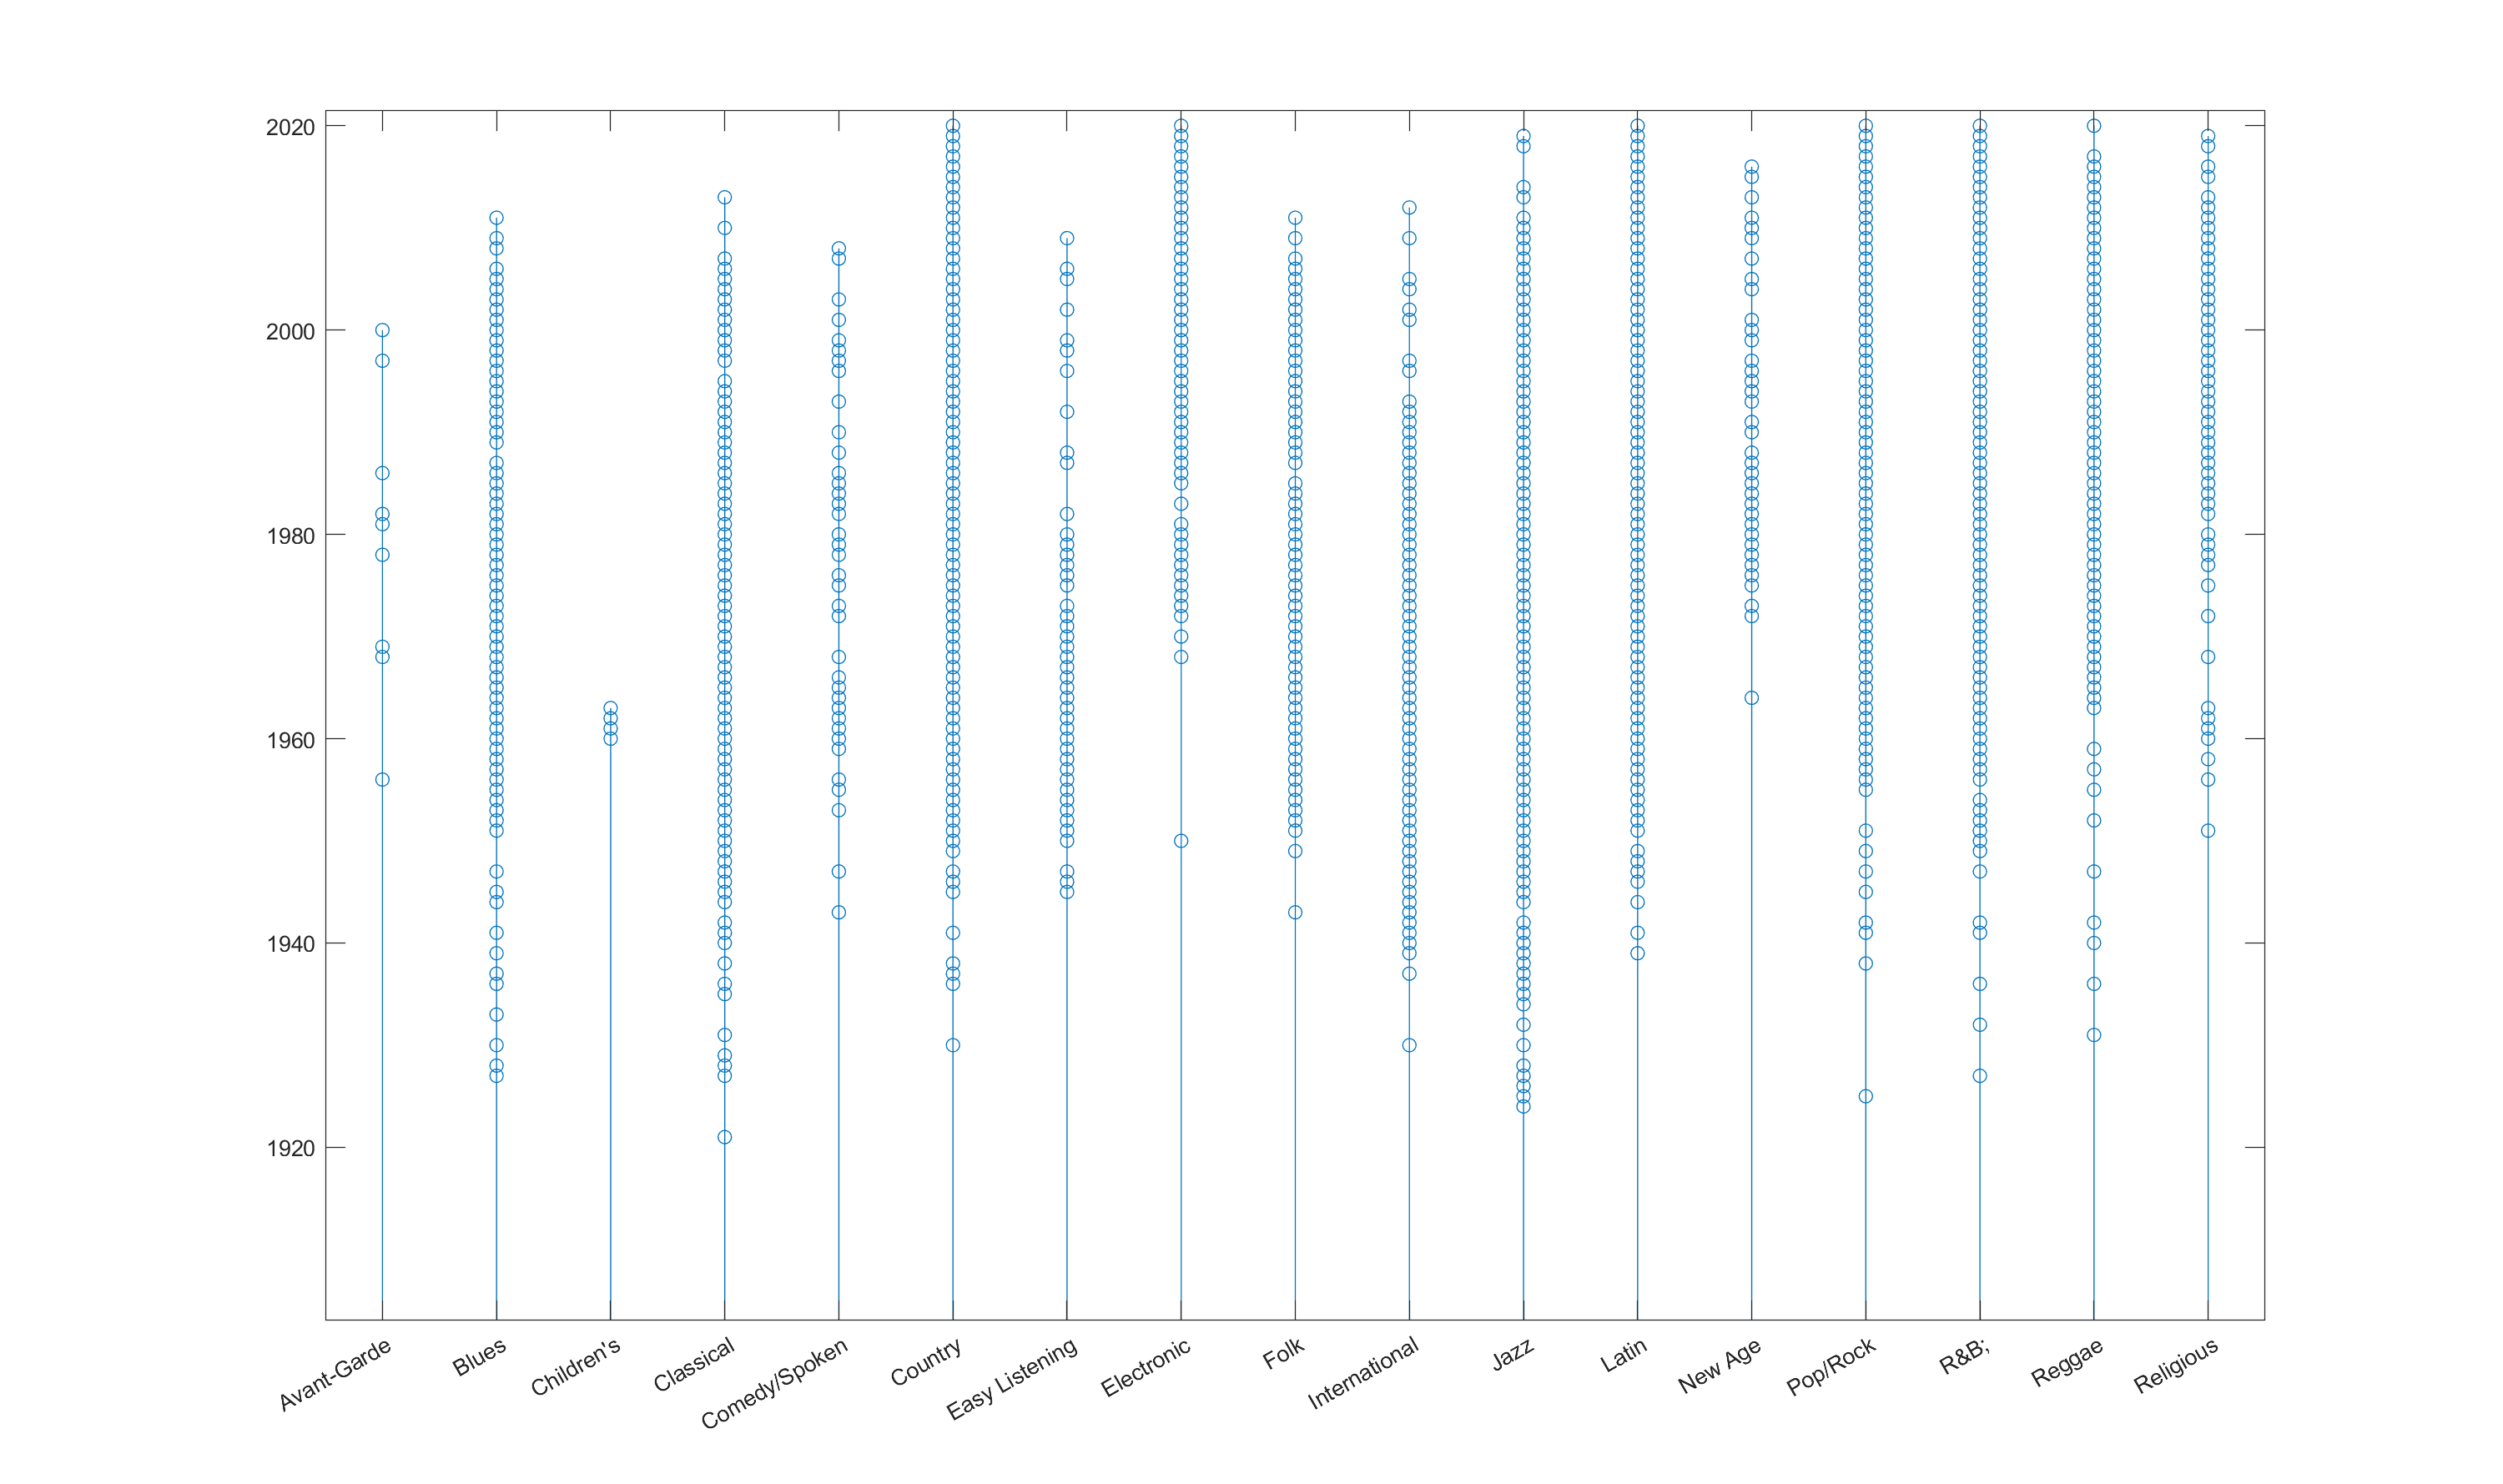
\includegraphics[scale=0.1]{Music21}
	\caption{Genre-Year Stem Chart}
\end{wrapfigure}
The stem chart was depicted according to the performance of works of each genre every year. Our team can find from the chart that \textit{classical, jazz, pop/rock, R \& B, country} and \textit{blue} came into being much earlier than others, leaving great and continuous impact on the novel genres from the mid to the terminal decade of 20th century. Many pieces music which are newly-born, including \textit{avant-garde, children's, electronic, new age} and \textit{reggae}, are still giving out their light and heat in this well-digitalized society, despite the weak prospects possessed by \textit{avant-garde, children's} and \textit{folk}.\\[2ex]\\
To analyze the musical characteristics of different genres, the indicators can be de-dimensioned with the factor analysis method shown in \textbf{4.1.3} and shown in the scatterplot chart in Figure 11(a).
\begin{figure}[h]
	\begin{subfigure}[Year-Characteristics Scatterplot Chart]
		{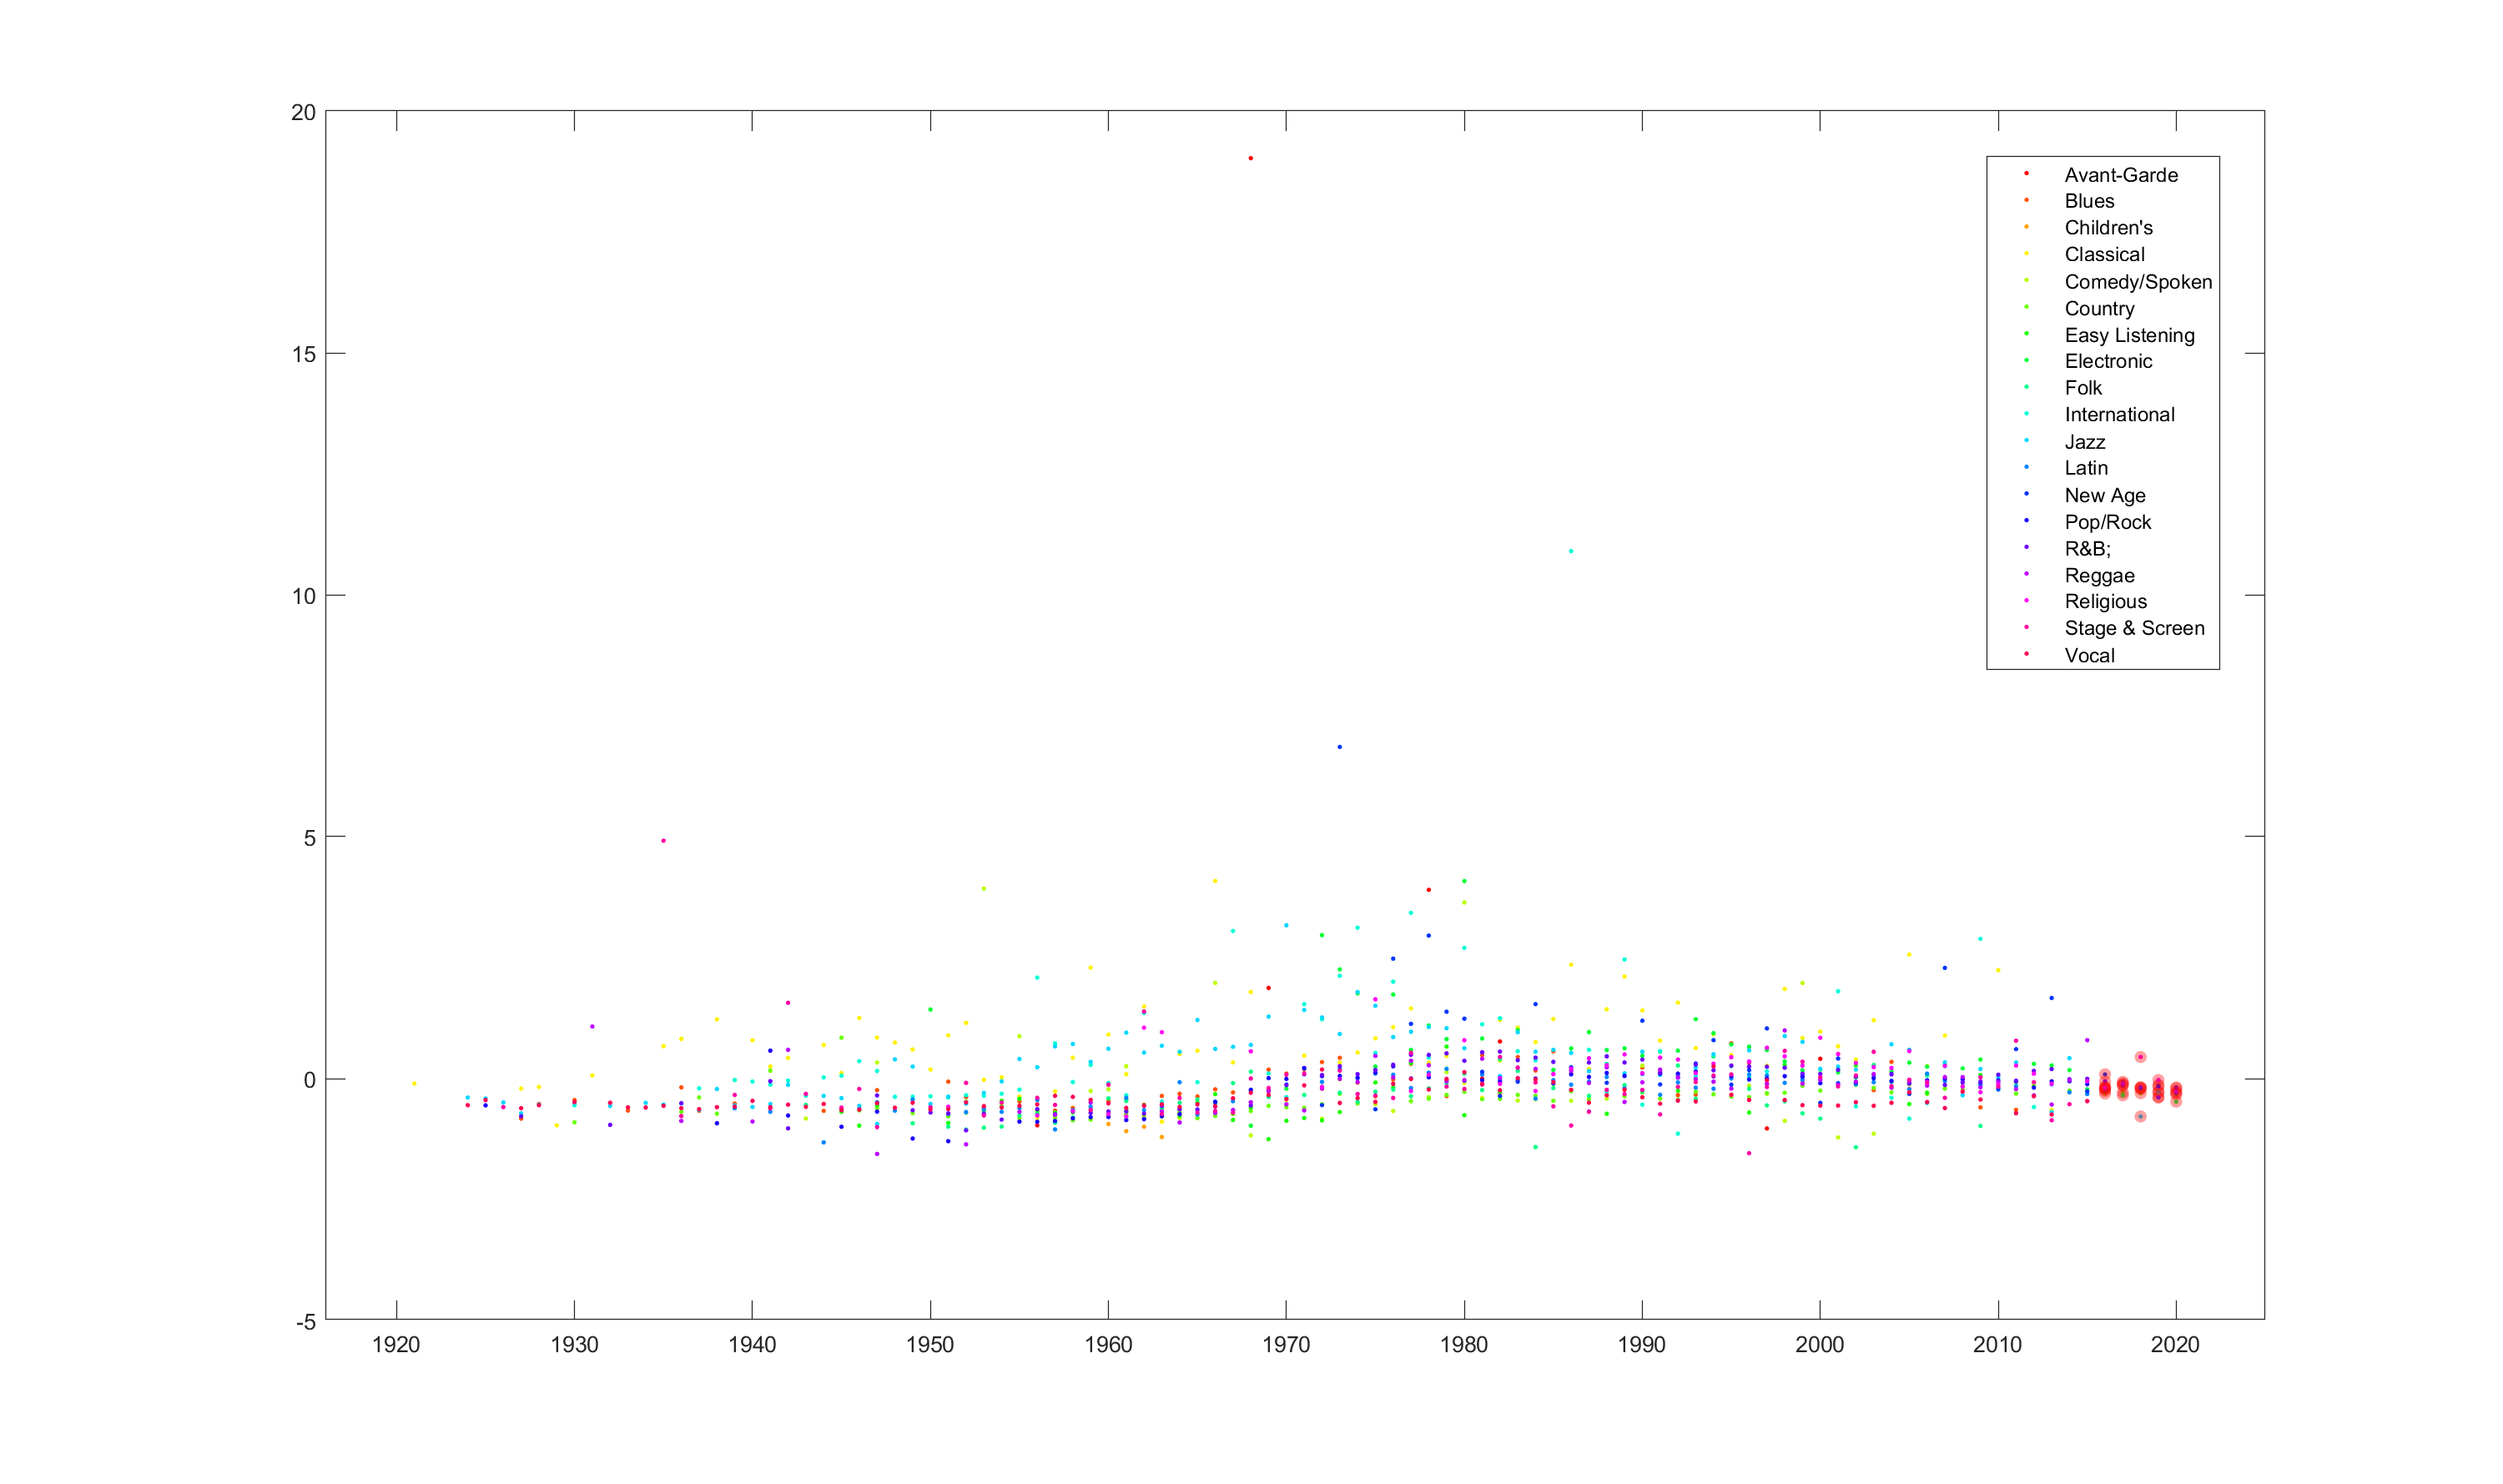
\includegraphics[scale=0.11]{Music22}}
	\end{subfigure}
	\begin{subfigure}[Year-Preferences Scatterplot Chart]
		{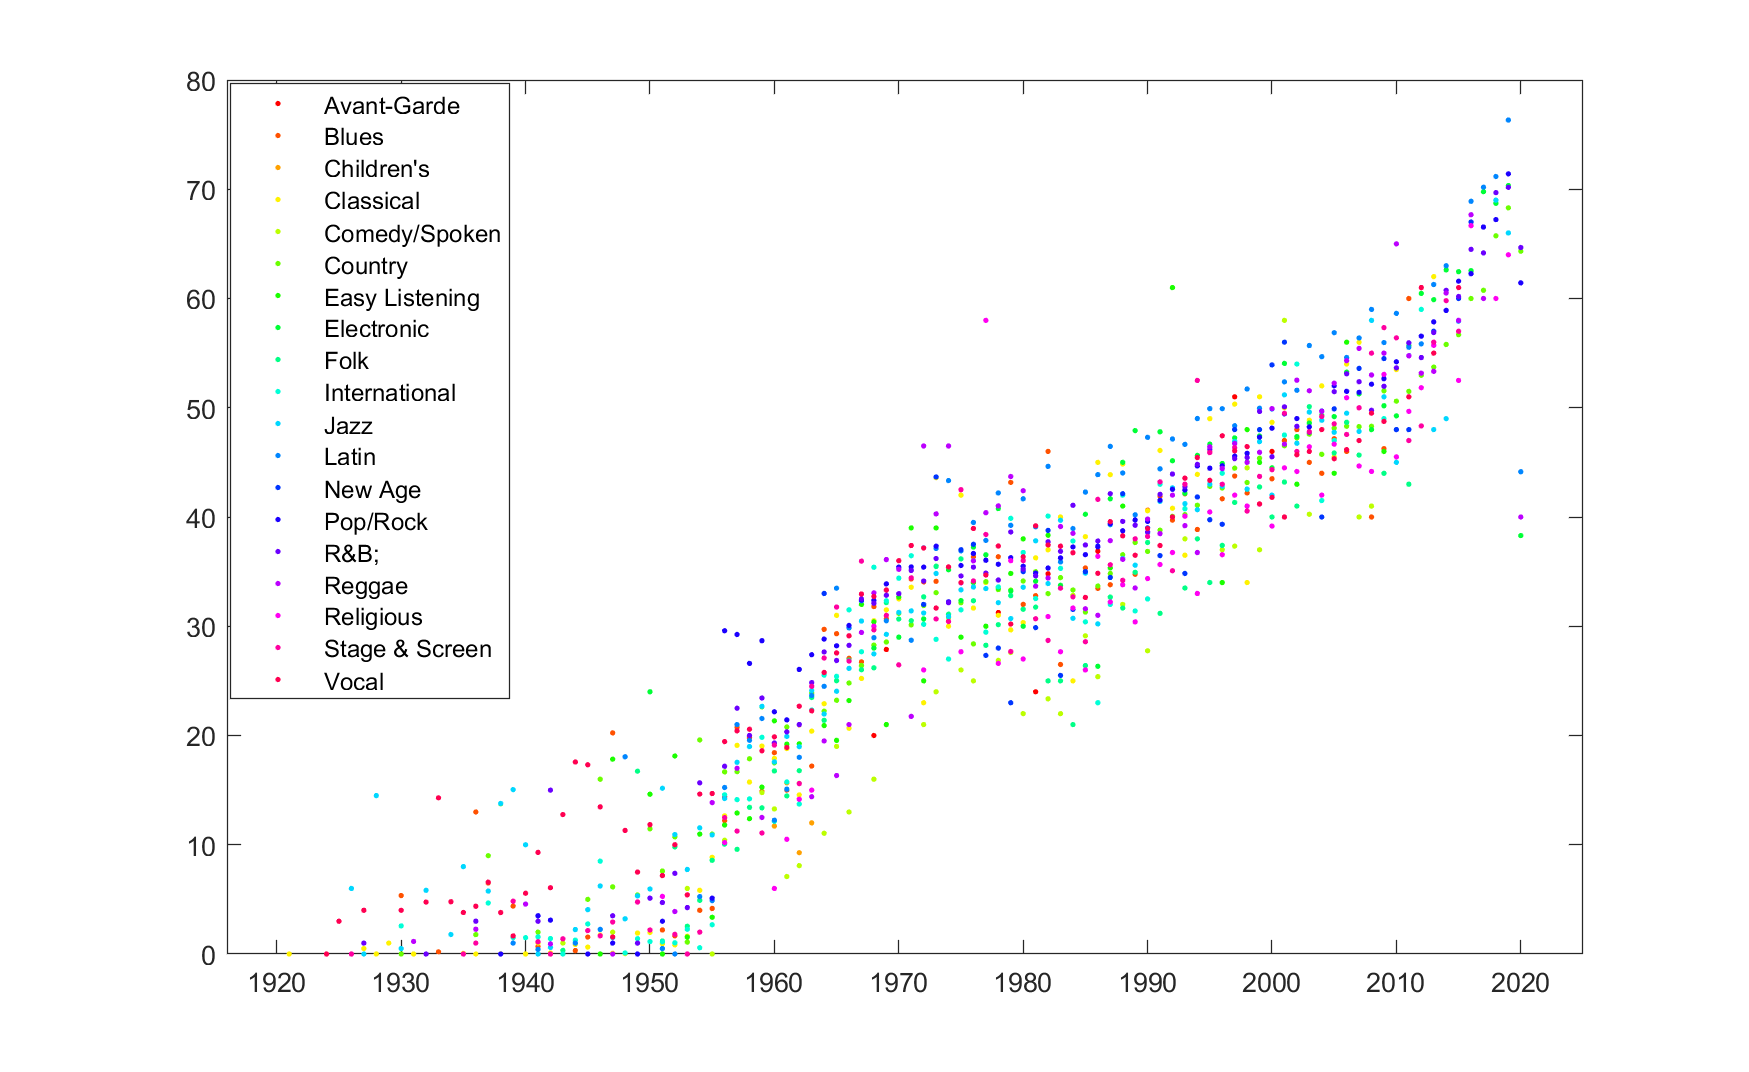
\includegraphics[scale=0.184]{Music23}}
	\end{subfigure}
	\caption{Scatterplot Charts for Development on Genres}
\end{figure}\\[5ex]
The chart shows that \textbf{some genres may play the leading role during a particular period}, with \textit{jazz, country, pop/rock} and \textit{Latin} stands out in the modern society. \textbf{Characteristics may make slight changes to follow the rhythm of the era.}\\[2ex]
The preferences of people in different decades are illustrated in Figure 11(b). The scatterplot chart can dynamically mirror the genres which enjoy popularity according to the time. Having taken historic, social, political and technological changes into consideration, we discovered that:
\begin{itemize}
	\item {\bfseries{\textit{Jazz} began to grow in the 1950s.}} The birth of \textit{jazz} can be attributed to the flow-in and the development of black-composed music and the mainstream of \textit{pop/rock} and \textit{blues}. The combination of movies and music redefined the existence of these special kinds of art. Making the whole thing better, the unique musical system \textit{jazz} constructed give birth to the development of modern pop music, \textit{blues, R \& B} and \textit{pop/rock} being the branches of it.
	\item {\bfseries{The \textit{booming of knowledge} era took place in the 1960s, inspiring the musicians of the significance of combining technology and their works.}} Branches of \textit{Electronics} and \textit{jazz} stood out, backing the implementation of the inspiration on to everyone's mind.
	\item {\bfseries{The voice for liberty and equality swept the air worldwide in the 1970s, the decade when music of all genres were enjoying their \textit{booming era}, pushing musicians to release the albums which call for freedom.}} Speech delivered by Martin Luther King, Jr. and Mao Zedong succeeded in igniting the souls of the revolutionists worldwide, encouraging them to compose tracks of radical feelings. The works expressing the true emotions of their authors soon gained great popularity worldwide, criticizing the cruel ruling system, the unfairness they're faced with and catching the ears of listeners. Bob Dylan, for example, began to get the key to hall of fame with the metal \textit{Blowing in the Wind}, which was born in that decade as well.
	\item The technology of Internet has made the spread of masterpieces easier for fans worldwide since the wide application of computers and other network-services-equipped devices. Existence of engineers for music and DJs has begun to turn more frequent, making the composition of tracks no longer limited to the inventions of inspiration. In other words, \textbf{A giant leap ahead in music has taken place in the late 1990s and the 21th century due to the small step forward in the development of computer.}
\end{itemize}
To conclude, {\textbf{development in genres can be accelerated by both external and internal factors. The overall trend of the development is to cater to the demands of people and to make full benefits of the cutting-edge technology at that age, absorbing the critical recipe for the popularity from works of other genres.}}
\clearpage
\section{Discussions}
\subsection{Sensitivity Analysis}
The results of PageRank Algorithm feature close links with the parameter $q$. In the second equation in \textbf{3.1}, $(1-q)$ represents possibility of self-changes under the condition that one node is spared from the influence of others. The PageRank Value in \textbf{3.1} is calculated under the condition $q=0.85$. The varying of PageRank Value, which follows the varying $q$, is as follows:
\begin{table}[h]
\centering
	\begin{tabular}{|c|c|c|c|c|c|}
		\hline
		q & Black Sabbath &Wishbone Ash &Iron Butterfly & Judas Priest &Deep Purple\\
		\hline
		0.05 &0.1958 &0.1958 &0.1959 &0.1920 &0.1958\\
		0.15 &0.1865 &0.1865 &0.1868 &0.1756 &0.1865\\
		0.25 &0.1755 &0.1775 &0.1763 &0.1588 &0.1755\\
		0.35 &0.1627 &0.1627 &0.1642 &0.1415 &0.1627\\
		0.45 &0.1477 &0.1477	 &0.1499	 &0.1235	 &0.1477\\
		0.55 &0.1301 &0.1301	 &0.1329 &0.1046 &0.1301\\
		0.65 &0.1095 &0.1095 &0.1127 &0.0847 &0.1095\\
		0.75 &0.0850 &0.0850 &0.0883 &0.0632 &0.0850\\
		0.85 &0.0558 &0.0558 &0.0584 &0.0399 &0.0558\\
		0.95 &0.0205 &0.0205 &0.0217	 &0.0141 &0.0205\\
		\hline
	\end{tabular}
\end{table}\\
It can be founded that the min-to-max order of PageRank Values remain the same when $q$ varies. The algorithm, thus, shows great stability in the sub-network.
\subsection{Strengths and weaknesses}
\subsubsection{Strengths}
\begin{itemize}
\item The network of influence can reveal the spread of the influence in it dynamically.
\item The criticality of every node can be evaluated from different perspectives thanks to employing \textsc{bc, dc} and PageRank Value.
\item High efficiency and excellent quality make it easier for analysis on ring-free map to be finished within a quite short time.
\item Our team have simplified the description of similarities among works in various parameters by de-dimensioning the stats and maintaining high describability.
\item Our team introduced {\textsc{cs}} at the condition of high accuracy of similarities so that the errors can hardly occur even if the data sets get larger.
\item Researches on a single artist can be transplanted for that on other artists and can reach safe conclusions as well.
\end{itemize}

\subsubsection{Weaknesses}
\begin{itemize}
	\item Complexity when applying \textsc{bc} may deny our this indicator when faced with piles of statistics.
	\item Extreme stats' existence may bring obvious fluctuation to the average.
	\item What we've founded are just limited to the statistics of reforms and influences among genres, which is much simpler than the actual situation of musical development.
	\item Inaccuracy may occur if time keeps going due to the assumption that value of parameters should not change with the time (included in \textbf{Assumption 1}).
\end{itemize}
\clearpage
\section{One-page Document to ICM Society}
The fence of these provided data sets should not restrict our models' usage; The genres in the entire world of music is not completely covered in these sets. The uncertainty, thus, stands out when the number of genres increases.\\[1ex]
Networks, revealing the link of influence among artists, may be increasingly complex thanks to the network of addition as the time keeps going. This in turn provides the networks opportunities to mirror the process of the spread existing in them. Our team are then able to explore the significance of every node in the network, finding out the composer of the musical revolution and the clubs which are leaving influences on each other. The link of influence among genres and the style of one genre can be also discovered with the help of the concerto of network.\\[1ex]
Faced with richer data, the network can still maintain the \textsc{scc} in the linear time complexity, employing Inc-\textsc{scc}, turning the network to \textsc{dag} and explore the spread of the influence in the networks. \textsc{dc} can be calculated within a quite high rate, while the calculation of \textsc{bc} requires the time of $O(|V||E|)$\textcolor{blue}{$^{[9]}$}. In other words, when the number of nodes and edges gets higher, the digits displaying on the timer should follow its path when it comes to calculation of \textsc{bc}. Common PageRank algorithm requires the time of $O(|V|^{2}t)$ ; but fortunately, plenty of algorithms have come to existence to optimize the solution of the PageRank Values\textcolor{blue}{$^{[10]}$}, which in turn gives us the chance to process statistics in larger scales, including the algorithm \textsc{mmsi}.\\[1ex]
Our team can take historic events and social reform into account and analyze distribution of artists of different genres and shifts on music characteristics for exploration of the reasons behind the rise and fall, the changes and the spread of the genres worldwide. Meanwhile, we can get a good command of the influences among culture, music and society by getting hold of the directions of spread of music shown in the network of influence and the related profiles. Our team can then step into the analysis of the reasons behind the great influences of some particular artists under the particular era, along with features of music characteristics of the musical masters in different decades.\\[1ex]
The ability of simulation for factors of similarities stands the test of richer data due to the de-dimensioning methods, including factors and cluster analysis. The analysis based on \textsc{cs} is suitable for spaces of any dimensions of vectors when it comes to researching on genres. Alternatively, we can still measure internal cohesion, figure out accurate range, power and trend of influences and even predict the coming-up revolutionary events in the near future when faced with data sets in a larger scale.\\[1ex]
The analysis of the network isn't only limited to the accordance to the changes of music characteristics, but also combined with the background of events at that time, including shifts in the social structure, scientific discoveries and revolutions. Taking all above into account, the distribution of artists of different genres can be explored in search of the reason behind the rise and fall of different genres, the styles of the masterpieces and the spread among regions. The richer the data is, the more history-related profiles we can get access to and the more evidences about analysis on the the correlation between cultural and musical spread, thus proving the discoveries regarding the reasons behind the strong influences of certain artists in one certain decade and the features of these musicians' masterpieces.\\[2ex]
All about the value of using our approach to understanding the influence of music through networks have been on display above. Our team is hoping that the report is able to compose a wonderful track of sonata which combines mathematics and music, and that the report can be adopted for further studies.
\clearpage
\begin{thebibliography}{99}
\addcontentsline{toc}{section}{References}
	\bibitem{1} Page.L. Brin.S. \emph{The anatomy of a large-scale hypertextual web search engine}. Computer Networks and ISDN Systems. 1998, 30: 107–117. ISSN 0169-7552. doi:10.1016/S0169-7552(98)00110-X. 
	\bibitem{2} {{\texttt{https://en.wikipedia.org/wiki/Centrality/}}}
	\bibitem{3} Tarjan, Robert (1972-06-01). \emph{Depth-first search and linear graph algorithms"}. SIAM Journal on Computing. 1(2): 146–160. doi:10.1137/0201010. ISSN 0097-5397.
	\bibitem{4} X.Liao, Y.Chen, Y.Zhang, et al. \emph{An efficient incremental strongly connected components algorithm for evolving directed graphs} (in Chinese). Sci Sin Inform, 2019, 49: 988–1004, doi: 10.1360/N112018-00125
	\bibitem{5} Kahn, Arthur B.(1962) \emph{Topological sorting of large networks}. Communications of the ACM, 5 (11): 558–562, doi:10.1145/368996.369025, S2CID 16728233.
	\bibitem{6} X.Shi, Y.Qian, F.Li. \emph{MS$^{2}$BC-a multi-view space structure-based clustering algorithm}. Journal of Southwest University, 2020, 42(11): 59-67. doi: 10.13718/j.cnki.xdzk.2020.11.007
	\bibitem{7} M.R.Silva. O.A.Carvalho. R.F.Guimarães. R.A.T.Gomes. C.R.Silva. \emph{Wheat planted area detection from the MODIS NDVI time series classification using the Nearest Neighbor Method calculated by the Euclidean Distance and Cosine Similarity Measures}. Geocarto International,2020,35(13).
	\bibitem{8} Y.Shao. \emph{Data similarity weight adjustment algorithm based on mathematical graph theory analysis}. Journal of Hunan University of Arts and Science (Science and Technology), 2021, 33(1): 20-24. doi: 10.3969/j.issn.1672-6146.2021.01.005
	\bibitem{9} U.Brandes. \emph{A faster algorithm for betweenness centrality}. Journal of Mathematical Sociology 25(2):163-177, 2001.
	\bibitem{10} Z.Yang. \emph{An effective accelerating iterative algorithm for computing PageRank}. Lanzhou University. 2019.
\end{thebibliography}
\clearpage
\section*{Appendix}
\addcontentsline{toc}{section}{Appendix}
\appendix
\hiddensection{Codes for Solving PageRank Values}
\lstset{ 
  backgroundcolor=\color{white},    
  basicstyle=\ttfamily,        
  breakatwhitespace=false,         
  breaklines=true,                 
  captionpos=b,                    
  commentstyle=\color{green},    
  deletekeywords={...},            
  escapeinside={\%*}{*)},          
  extendedchars=true,               
  frame=single,	                   
  keepspaces=true,                 
  keywordstyle=\color{blue},       
  language=Octave,                 
  morekeywords={*,...},            
  numbers=left,                    
  numbersep=5pt,                   
  numberstyle=\tiny\color{gray}, 
  rulecolor=\color{black},
  showspaces=false,                
  showstringspaces=false,          
  showtabs=false,                  
  stepnumber=1,                    
  stringstyle=\color{orange},     
  tabsize=2,	                   
  title=\lstname                   
}
\begin{lstlisting}[language=C++]{PageRank.cpp}
#include<bits/stdc++.h>
using namespace std;
const int maxn = 17;
int g[10][10], n = 5, cnt;
double PR[10], S[10][10], deg[10], a = 0.7, dv;
bool mul(){
    cnt++;
    if (cnt > 100) return 1;
    double res[10], change = 0;
    for (int i = 1; i <= 5; i++) {res[i] = 0;}
    for (int i = 1; i <= 5; i++) {
        for (int j = 1; j <= 5; j++) {
            if (S[j][i] == 1) {res[i] += a * PR[j] / deg[j];}
        }
        res[i] += dv;
        change += abs(PR[i] - res[i]);
    }
    for (int i = 1; i <= n; i++) {PR[i] = res[i];}
    if (change < 0.0001) {return true;}
    return false;}
int main() {
    g[1][4]=g[2][4]=g[3][5]=g[3][2]=g[3][1]=g[4][3]=g[5][4]=1;
    deg[1] = 1; deg[2] = 1; deg[3] = 3; deg[4] = 1; deg[5] = 1;
    for (int i = 1; i <= 5; i++) {
        for (int j = 1; j <= 5; j++) {
            if (i != j) {
                if (deg[i] != 0 && g[i][j]){S[i][j] = 1.0/deg[i];}
                else {S[i][j] = 0.2;
                    deg[i] = 5;
                    for (int k = 1; k <= 5; k++) S[i][j] = 1;}
            }
        }
        PR[i] = 0.2;dv = (1.0-a) / 5;
    }
    while (!mul()) ;
    for (int i = 1; i <= 5; i++) {printf("%.5lf\n", PR[i]);}
}
\end{lstlisting}
\clearpage
\hiddensection{Codes for Factor Analysis (Key Part)}
\lstset{ 
  backgroundcolor=\color{white},    
  basicstyle=\ttfamily,        
  breakatwhitespace=false,         
  breaklines=true,                 
  captionpos=b,                    
  commentstyle=\color{green},    
  deletekeywords={...},            
  escapeinside={\%*}{*)},          
  extendedchars=true,               
  frame=single,	                   
  keepspaces=true,                 
  keywordstyle=\color{blue},       
  language=Octave,                 
  morekeywords={*,...},            
  numbers=left,                    
  numbersep=5pt,                   
  numberstyle=\tiny\color{gray}, 
  rulecolor=\color{black},
  showspaces=false,                
  showstringspaces=false,          
  showtabs=false,                  
  stepnumber=1,                    
  stringstyle=\color{orange},     
  tabsize=2,	                   
  title=\lstname                   
}
\begin{lstlisting}[language=Matlab]{FactorAnalysis.m (Partial)}
	clc
clear all
A=xlsread(' C:\Users\..\Desktop\ influence_data.xlsx ');
a=size(A,1);
b=size(A,2);
for i=1:b
    SA(:,i)=(A(:,i)-mean(A(:,i)))/std(A(:,i));
end
CM=corrcoef(SA);
[V,D]=eig(CM);
for j=1:b
    DS(j,1)=D(b+1-j,b+1-j);
end
for i=1:b
    DS(i,2)=DS(i,1)/sum(DS(:,1));
    DS(i,3)=sum(DS(1:i,1))/sum(DS(:,1));
end
T=0.9;
for k=1:b
    if DS(k,3) >= T
        com_num=k;
        break;
    end
end
for j=1:com_num
    PV(:,j)=V(:,b+1-j);
end
new_score=SA*PV;
for i=1:a
    total_score(i,1)=sum(new_score(i,:));
    total_score(i,2)=i;
end
result_report=[new_score,total_score];
result_report=sortrows(result_report,-4);
\end{lstlisting}
\clearpage
\hiddensection{Codes for Shrinking Points (Key Part)}
\lstset{ 
  backgroundcolor=\color{white},    
  basicstyle=\ttfamily,        
  breakatwhitespace=false,         
  breaklines=true,                 
  captionpos=b,                    
  commentstyle=\color{green},    
  deletekeywords={...},            
  escapeinside={\%*}{*)},          
  extendedchars=true,               
  frame=single,	                   
  keepspaces=true,                 
  keywordstyle=\color{blue},       
  language=Octave,                 
  morekeywords={*,...},            
  numbers=left,                    
  numbersep=5pt,                   
  numberstyle=\tiny\color{gray}, 
  rulecolor=\color{black},
  showspaces=false,                
  showstringspaces=false,          
  showtabs=false,                  
  stepnumber=1,                    
  stringstyle=\color{orange},     
  tabsize=2,	                   
  title=\lstname                   
}
\begin{lstlisting}[language=c++]{ShrinkingPoints.cpp (Partial)}
void tarjan(int u){
	dfn[u] = low[u] = ++tot;
	instack[u] = 1; stack[++top] = u;
	for (int i = head[u]; ~i; i = e[i].nxt) {
		int v = e[i].v;
		if (!dfn[v]) {
			tarjan(v);
			low[u] = min(low[u], low[v]);
		} else if (instack[v]) {
			low[u] = min(low[u], dfn[v]);
		}
	}
	if (dfn[u] == low[u]) {
		cnt++; int v = 0;
		do {
			v = stack[top--]; instack[v] = 0;
			col[v] = cnt; scc[cnt].push_back(v);
		} while (v != u);
	}
}
\end{lstlisting}

\end{document}
\end